
% This is for rubber to remove slides.vrb automatically created by tikz
% rubber: watch $job.vrb
% rubber: clean $job.vrb

% \documentclass[xcolor=dvipsnames,12pt]{beamer}
% \documentclass[draft,handout,xcolor=dvipsnames]{beamer}
\documentclass[handout,xcolor=dvipsnames]{beamer}
% \documentclass[draft,xcolor=dvipsnames]{beamer}
% \documentclass[xcolor=dvipsnames]{beamer}

% Commands
\newcommand{\DSU}{{\sc Jvolve}}
\newcommand{\JikesRVM}{Jikes RVM}

\newcommand{\ShowTOC}[1][currentsection,currentsubsection]{%
\begin{frame}{Outline}%
  \tableofcontents[#1]%
  % You might wish to add the option [pausesections]%
\end{frame}%
}

% Include packages
\usepackage{colortbl}
\usepackage[absolute,overlay]{textpos}
\usepackage[normalem]{ulem}
\usepackage[override]{cmtt}
\usepackage{graphicx}
\usepackage{ifdraft}
\usepackage{tikz}
\usetikzlibrary{arrows,backgrounds}

% Include customized theme

\mode<beamer> {
  % But using Burnt orange instead of the blue used by that there. Changing
  % the beamercolor "structure" to burnt orange pretty much changes
  % everything. Really cool!!!
%   \definecolor{burntorange}{HTML}{CC5500}
%   \usecolortheme[named=burntorange]{structure}

%   The Copenhagen theme with innertheme [shadow=true] and rounded
%   \useinnertheme[shadow=true]{rounded}
  \usetheme{Madrid}
  \setbeamercolor{section in head/foot}{parent=palette tertiary}
  \setbeamercolor{subsection in head/foot}{parent=palette secondary}
  \setbeamercolor{date in head/foot}{parent=palette primary}
%   \setbeamersize{text margin left=1.5em,text margin right=1.5em}

%   The Warsaw theme and our customization
%   \usetheme{Warsaw}
%   \setbeamercolor*{palette quaternary}{use=structure,fg=white,bg=structure.fg!55!black}
%   \useoutertheme{split}

%   The Madrid theme and our customization
%   \usetheme[secheader]{Madrid}
%   \setbeamercolor*{subsection in head/foot}{parent=palette secondary}
%   \setbeamercolor*{palette quaternary}{use=structure,fg=white,bg=yellow}

  \setbeamercovered{transparent}

  \setbeamertemplate{footline}{%
   \begin{beamercolorbox}[wd=\paperwidth,ht=2.25ex,dp=1ex,right]{date in head/foot}%
     \usebeamerfont{date in head/foot}Slide \insertframenumber{}\hspace*{2ex}%
   \end{beamercolorbox}}

   \setbeamertemplate{sections/subsections in toc}[ball unnumbered]{}

   \setbeamertemplate{navigation symbols}{}
%   \setbeamertemplate{bibliography item}[text]
}

\mode<handout> {
  \usepackage{pgfpages}
  \input{theme/six-on-one.sty}
  \pgfpagesuselayout{8 on 1}[letterpaper,border shrink=1mm]
  \usetheme{default}
%   \setbeamertemplate{footline}[page number]
  \setbeamercolor{background canvas}{bg=black!5}
  \setbeamertemplate{footline}{%
   \begin{beamercolorbox}[wd=\paperwidth,ht=2.25ex,dp=1ex,right]{date in head/foot}%
     \usebeamerfont{date in head/foot}Slide \insertframenumber{}\hspace*{2ex}%
   \end{beamercolorbox}}
}

% If you have a file called "university-logo-filename.xxx", where xxx
% is a graphic format that can be processed by latex or pdflatex,
% resp., then you can add a logo as follows:

% \pgfdeclareimage[height=0.5cm]{university-logo}{university-logo-filename}
% \logo{\pgfuseimage{university-logo}}

% Delete this, if you do not want the table of contents to pop up at
% the beginning of each subsection:
% \AtBeginSubsection[]
% \AtBeginSection[]
% {
%   \begin{frame}<beamer>{Outline}
%     \tableofcontents[currentsection,currentsubsection]
%   \end{frame}
% }

% If you wish to uncover everything in a step-wise fashion, uncomment
% the following command: 

%\beamerdefaultoverlayspecification{<+->}


\title[Dynamic Software Updates in Java]
{Dynamic Software Updates in Java:\\ A VM-centric approach}

% \subtitle
% {Presentation Subtitle} % (optional)

\author[Suriya Subramanian]{%
Suriya Subramanian\\
Advisor: Kathryn S. McKinley}
\institute[The University of Texas at Austin] % (optional, but mostly needed)
{
  Department of Computer Sciences\\
  The University of Texas at Austin
}

\date[Short Occasion]
{July 21, 2008\\
Ph.D. Oral Proposal}
\subject{Ph.D. Oral Proposal}

\begin{document}


{
% UT seal got from http://www.utexas.edu/visualguidelines/vg_seals.html
\setbeamertemplate{navigation symbols}{}
\setbeamertemplate{headline}{}
\setbeamertemplate{footline}{}
% \mode<beamer>{
% \setbeamertemplate{background canvas}{{\color{bg}\vrule width 0\paperwidth height \paperheight}%
% 
\includegraphics[keepaspectratio=true,clip=true,trim=380pt 550pt 0pt 0pt]{theme/ut-seal}}
% }
\begin{frame}
  \titlepage
\end{frame}
}



% {
% \setbeamertemplate{headline}{}
% \setbeamertemplate{footline}{}
% \setbeamertemplate{navigation symbols}{}
% \begin{frame}
% \begin{block}{}
% \begin{quote}
% The only thing that is constant is change.\\
% \hfill Heraclitus of Ephesus
% \end{quote}
% \end{block}
% \end{frame}
% }

% \section{Introduction}
% \subsection{Motivation}
\begin{frame}{Motivation}%{A Sub-title is optional}
\begin{itemize}
\item Software applications change all the time
\item Deployed systems must be updated with bug fixes, new features
\item Updating typically involves: stop, apply patch, restart
% \vspace{1ex}
% \begin{center}\begin{Huge}Updating $\Rightarrow$ Downtime\end{Huge}\end{center}
\item Not desirable
  \begin{itemize}
    \item Safety concerns
    \item Revenue loss
    \item Inconvenience
  \end{itemize}
\end{itemize}
% \item Might not be affordable for some applications
%   \begin{itemize}
%   \item Applications that retain state that cannot be externalized
%   \end{itemize}
\end{frame}

\begin{frame}{Dynamic software updating}%{A Sub-title is optional}
\vspace*{-3mm}%
\begin{center}%
\includegraphics[scale=0.73]{images/process-state/both-process-state}%
\end{center}%
\end{frame}

\begin{frame}{Dynamic updating systems}%{A Sub-title is optional}
\begin{itemize}
\item Special-purpose architectures, application-specific solutions exist
\item General-purpose solutions gaining strength
  \begin{itemize}
  \item K42, Ksplice for OS updates
  \item Polus, Ginseng for C applications
  \end{itemize}
\item Not for managed languages
\end{itemize}
\end{frame}

% \begin{frame}{Motivation}%{A Sub-title is optional}
% \begin{itemize}
% \item Software applications change all the time
% \item Deployed systems need to be updated
% \item Some systems cannot afford downtime (safety concerns, revene loss),
% many systems perfer to avoid downtime (inconvenience)
% \item Stopping, updating and restarting deployed systems is not ideal
% \item Neither is delaying critical updates
% \end{itemize}
% \end{frame}

% \begin{frame}{Motivation}%{A Sub-title is optional}
% \begin{itemize}
% \item 75\% of downtime in high-availablity applications is for planned
% maintenance
% \uncover<2->{
% \item Personal operating system
% \item Enterprise applications
% \item Telecommunication, transportation systems
% % \uncover<3->{
% % \item Even a cache with lots of state
% %   \begin{itemize}
% %   \item LinkedIn.com architecture\footnote{\scriptsize{\url{http://hurvitz.org/blog/2008/06/linkedin-architecture}}}
% %   \item ``The Cloud'': In memory representation of the LinkedIn network graph
% %   \item Network size - 22M nodes, 120M edges
% %   \item Rebuilding an instance takes 8 hours
% %   \end{itemize}
% % }
% }
% \end{itemize}
% \end{frame}

% % \subsection{Solutions}
% \begin{frame}{Conventional solutions to avoid downtime}%{A Sub-title is optional}
% \begin{itemize}
% \item Move state out of the process, for instance databases
% \item Use multiple processes, and do a rolling update
% \end{itemize}
% \uncover<2>{
% \begin{itemize}
% \item Not always possible
% \item Restricted to specific application domains
% % \item DSU is a generic solution
% \end{itemize}
% }

% \begin{frame}{Dynamic Software Updating}%{A Sub-title is optional}
% Updating state of a process on the fly
% \begin{itemize}
% \item Special purpose techniques/architectures work, but we want a general
% solution
% \item 
% \end{itemize}
% \end{frame}

%   \begin{itemize}
%   \item State stored externally, for instance databases
%   \item Redundant systems: start a new process and stop this one
%   \item Not always possible
%   \end{itemize}
% \item<2-> Dynamic Software Updating (DSU)
%   \begin{itemize}
%     \item Update process state without restarting application
%     \item Non-redundant systems benefit as well
%     \item Decouples fault-tolerance from software updating
%   \end{itemize}
% \end{frame}

% \begin{frame}{Process state}%{A Sub-title is optional}
% \vspace*{-2ex}\includegraphics[scale=0.72]{images/process-state}
% \end{frame}

% \begin{frame}{DSU requirements}%{A Sub-title is optional}
% % \begin{center}
% % A Dynamic Software Updating solution should \emph{ideally} be
% % {\bf safe}, {\bf flexible}, and {\bf efficient}.
% % \end{center}
% \begin{description}
% \item[Safe] Updating is as correct as starting from scratch
% \item[Flexible] Support changes encountered in practice
% \item[Efficient] No performance impact
% \end{description}
% \end{frame}

% \begin{frame}{State of the art}%{A Sub-title is optional}
% Significant progress for C
% \begin{itemize}
% \item Server feature upgrades
%   \begin{itemize}
%   \item Ginseng \cite{neamtiu06dsu}
%   \item POLUS \cite{chen:icse07}
%   \end{itemize}
% \item Security patches: OPUS \cite{altekar05opus}
% \item Operating system upgrades
%   \begin{itemize}
%   \item K42 \cite{K42reconfig}
%   \item DynAMOS \cite{dynamos_eurosys_07}
%   \item LUCOS \cite{chen06vee}
%   \item Ksplice \cite{Ksplice}
%   \end{itemize}
% \end{itemize}
% % \item<2-> Primitive support for managed languages
% %   \begin{itemize}
% %   \item Very restrictive
% %   \item Space and time overheads
% %   \item Not proven on realistic applications
% %   \end{itemize}
% \end{frame}

% \begin{frame}{DSU opportunity for managed languages}%{A Sub-title is optional}
% DSU Solutions for C/C++ typically
% \begin{itemize}
% \item Require special compilation
% \item Statically/dynamically insert indirection for function calls
% \item Restrict structure updates, require extra allocation
% \item Impose space/time overheads on normal execution
% \item Make type-safety for updates difficult
% \item Not multi-threaded
% \end{itemize}
% \end{frame}

% \begin{frame}{Possible DSU solutions}%{A Sub-title is optional}
% Achieve DSU support by
% \begin{itemize}
% \item Making the application DSU-aware
% \item Special recompilation
% \item A class loader based colution 
% \item DSU support in the VM
% \end{itemize}
% \end{frame}

% \begin{frame}{Related work}%{A Sub-title is optional}
% \begin{itemize}
% \item Custom class loader solutions:\\Eisenbach and Barr, Milazzo et al.
% \item Source-to-source translation: Orso et al.
% \item VM-based solutions: JDrums, Dynamic Virtual Machine (DVM)
% \item In a persistent object store: Boyapati et al.
% \end{itemize}
% \uncover<2>{
% \begin{itemize}
% \item Limited, not flexible
% \item Restricted data-transformation model (like requiring {\em encapsulation} based
% on {\em ownership types})
% \item Overhead during normal execution
% \end{itemize}
% }
% \end{frame}

% \begin{frame}{Existing solutions for managed languages}%{A Sub-title is optional}
% \begin{itemize}
% \item VM-based solutions
%   \begin{itemize}
%   \item JDrums \cite{ritzau00dynamic}, DVM \cite{Mala00a}
%   \item Not well evaluated
%   \item Provide an interface similar to \DSU{}
%   \item Perform lazy updates
%   \item Overheads during normal execution
%   \end{itemize}
% \item Standard VM with DSU support
%   \begin{itemize}
%   \item DJVCS \cite{BarrE03}, DUSC \cite{orso:java}, \cite{Milazzo05updates}
%   \item Special classloaders, compilers
%   \item Very restrictive
%   \item Space/time overheads
%   \end{itemize}
% \end{itemize}
% 
% \end{frame}

% \begin{frame}{Related work}%{A Sub-title is optional}
% Nobody can beat us.
% \end{frame}

\begin{frame}{Our solution}%{A Sub-title is optional}
\begin{itemize}
\item \DSU{} - a Java Virtual Machine with DSU support
% \item Built on top of Jikes RVM, a Java-in-Java VM
\item Key insight: Extend existing VM services
%   \begin{itemize}
%   \item Classloading
%   \item Bytecode verification%\footnote{Jikes RVM does not have a bytecode verifier}
%   \item Thread synchronization
%   \item JIT Compilation
%   \item On-stack replacement
%   \item Garbage collection
%   \end{itemize}
\item No DSU-related overhead during normal execution
\item Support updates to real world applications
\begin{block}{}
\emph{Dynamic software updating in managed languages can be achieved in a
{\bf safe}, {\bf flexible} and {\bf efficient} manner by naturally extending existing VM
services.}
\end{block}

\begin{block}{}
\emph{DSU support should be a standard feature of future VMs.}
\end{block}
\end{itemize}
\end{frame}

% \begin{frame}{Contribution}%{A Sub-title is optional}
% \setbeamercovered{invisible}
% \begin{block}{}
% \emph{Dynamic software updating in managed languages can be achieved in a
% {\bf safe}, {\bf flexible} and {\bf efficient} manner by naturally extending existing VM
% services.}
% \end{block}
% 
% \begin{block}<2->{Corollary}
% \emph{DSU support should be a standard feature of future VMs.}
% \end{block}
% \end{frame}


\section{\DSU}
\ShowTOC[currentsection]

\begin{frame}{Developer's view of \DSU{}}%{A Sub-title is optional}
\begin{center}%
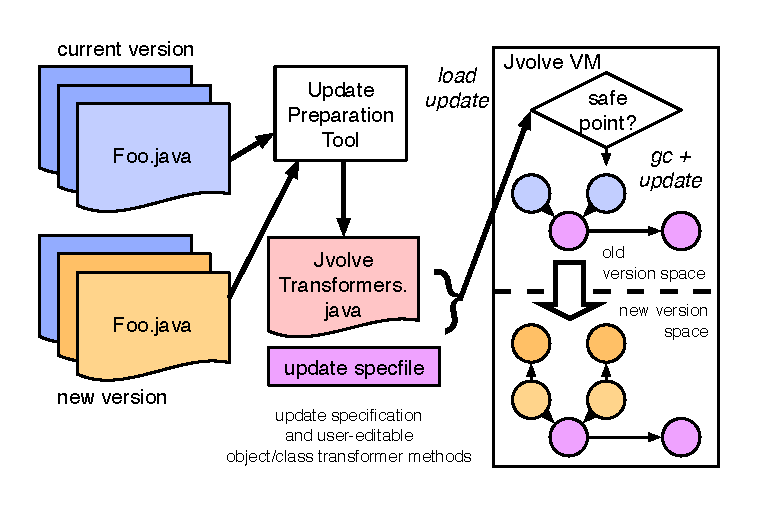
\includegraphics[width=0.93\paperwidth]{images/system}%
\end{center}%
\end{frame}

\begin{frame}{VM's view of DSU}%{A Sub-title is optional}
\begin{itemize}
\item Update happens in one fell swoop
\item Simple to reason about
\item Code
  \begin{itemize}
  \item Old code before the update
  \item New code after the update
  \end{itemize}
\item Data
  \begin{itemize}
  \item \emph{Representation consistency} (all values of a type \\
        correspond to the latest version)
  \item Support a transformation function to convert objects to conform to
        their new definition
  \end{itemize}
\end{itemize}
\end{frame}

\subsection{Developer's role}

\begin{frame}{Division of Labor}%{A Sub-title is optional}
\begin{itemize}
\item Developer
  \begin{itemize}
  \item Write the old and new versions
  \item Write class/object transformation functions for classes that
        changed (optional)
  \item Testing (both the application and the update)
  \end{itemize}
\item \DSU{} system
  \begin{itemize}
  \item Update Preparation Tool (UPT) compares versions and presents the
        update to the \DSU{} VM.
  \item \DSU{} VM handles the update
  \end{itemize}
\end{itemize}
\end{frame}

\begin{frame}{Supported updates}%{A Sub-title is optional}
\begin{itemize}
\item Changes within the body of a method
\item Class signature updates
  \begin{itemize}
  \item Add, remove, change the type signature of fields and methods
  \end{itemize}
\item Changes can occur at any level of the class hierarchy
\end{itemize}
\end{frame}

\ShowTOC

\newcommand{\ExampleCodeSize}{footnotesize}
\begin{frame}[fragile,shrink=5]{Example of an update (JavaEmailServer)}%{A Sub-title is optional}
\begin{\ExampleCodeSize}
\begin{verbatim}
  public class User {
    private final String username, domain, password;
    private String[] forwardAddresses;
    public User(...) {...}
    public String[] getForwardedAddresses() {...}
    public void setForwardedAddresses(String[] f) {...}
  }

  public class ConfigurationManager {
    private User loadUser(...) {
       ...
       User user = new User(...);
       String[] f = ...;
       user.setForwardedAddresses(f);
       return user;
    }
  }




\end{verbatim}
\end{\ExampleCodeSize}
\end{frame}

% \begin{frame}[fragile,shrink=5]{Example of an update (JavaEmailServer)}%{A Sub-title is optional}
% \begin{\ExampleCodeSize}
% \begin{semiverbatim}
% public class User \{
%   private String username, domain, password;
%   private \sout{String[]} EmailAddress[] forwardAddresses;
%   public \sout{String[]} EmailAddress[] getForwardedAddresses() \{...\}
%   public void setForwardedAddresses(\sout{String[]} EmailAddress[] f) \{...\}
% \}
% 
% public class ConfigurationManager \{
%   private User loadUser(...) \{
%      ...
%      User user = new User(...);
%      \sout{String[]} EmailAddress[] f = ...;
%      user.setForwardedAddresses(f);
%      return user;
%   \}
% \}
% 
% \end{semiverbatim}
% \end{\ExampleCodeSize}
% \end{frame}

\begin{frame}[fragile,shrink=5]{Example of an update (JavaEmailServer)}%{A Sub-title is optional}
\newcommand{\removed}[1]{\textcolor{red}{- #1}}
\newcommand{\addedxx}[1]{\textcolor{OliveGreen}{+ #1}}
\begin{\ExampleCodeSize}
\begin{semiverbatim}
  public class User \{
    private final String username, domain, password;
\removed{  private String[] forwardAddresses;}
\addedxx{  private EmailAddress[] forwardAddresses;}
    public User(...) {...}
\removed{  public String[] getForwardedAddresses() \{...\}}
\addedxx{  public EmailAddress[] getForwardedAddresses() \{...\}}
\removed{  public void setForwardedAddresses(String[] f) \{...\}}
\addedxx{  public void setForwardedAddresses(EmailAddress[] f) \{...\}}
  \}

  public class ConfigurationManager \{
    private User loadUser(...) \{
       ...
       User user = new User(...);
\removed{     String[] f = ...;}
\addedxx{     EmailAddress[] f = ...;}
       user.setForwardedAddresses(f);
       return user;
    \}
  \}
\end{semiverbatim}
\end{\ExampleCodeSize}
\end{frame}

\begin{frame}{Object Transformers}%{A Sub-title is optional}
\begin{itemize}
\item ``Transform'' objects to correspond to the new version
\item Functions generated by the Update Preparation Tool (UPT)
\item Accept old object and new objects as parameters
\item Default transformer copies old fields and initializes new ones to
\texttt{null}
\item User can optionally modify these functions
\end{itemize}
\end{frame}

\begin{frame}[fragile,shrink=5]{Object Transformers}%{A Sub-title is optional}
\mode<beamer> {
\begin{textblock*}{46mm}[0,0](79mm,26mm)
\begin{block}{}
Stub generated by UPT for the old version
\end{block}
\end{textblock*}
\only<1>{
\begin{textblock*}{46mm}[0,0](79mm,48mm)
\begin{block}{}
Default transformer copies old fields, initializes new ones to
\texttt{null}
\end{block}
\end{textblock*}}
}
\begin{small}
\begin{semiverbatim}
public class v131_User \{
  private final String username, domain, password;
  private String[] forwardAddresses;
\}
public class JvolveTransformers \{
 ...
 public static void jvolveClass(User unused) \{\}
 public static void jvolveObject(User to, v131_User from) \{
    to.username = from.username;
    to.domain = from.domain;
    to.password = from.password;
    // to.forwardAddresses = null;
    \uncover<2>{int len = from.forwardAddresses.length;
    to.forwardAddresses = new EmailAddress[len];
    for (int i = 0; i < len; i++) \{
      to.forwardAddresses[i] =
        new EmailAddress(from.forwardAddresses[i]);
}\}\}\}

\end{semiverbatim}
\end{small}
\end{frame}

\newcommand{\JvolveTimeLine}[5]{
\begin{center}
\begin{tikzpicture}[auto]
  \tikzstyle{block}=[
    font=\tiny,
    rectangle,
    draw=structure.fg,
    thick,
    text width=1.2cm,
    text badly centered,
    rounded corners,
    minimum height=2em,
  ]
  \tikzstyle{current}=[fill=structure.fg!20, ]
  \tikzstyle{line}=[draw, thick, -latex',]
  \tikzstyle{every path}=[line]
  \matrix [column sep=5mm,row sep=7mm,ampersand replacement=\&] {
    \node [block,#1] (0) {\hyperlink{offline}{Offline tool}};          \&
    \node [block,#2] (1) {\hyperlink{suspend}{Suspend application}};   \&
    \node [block,#3] (2) {\hyperlink{classload}{Install new classes}}; \&
    \node [block,#4] (3) {\hyperlink{transform}{Transform objects}};   \&
    \node [block,#5] (4) {Resume application};                         \\
  };
  \path (0) -- (1);
  \path (1) -- (2);
  \path (2) -- (3);
  \path (3) -- (4);
\end{tikzpicture}
\end{center}
}


\subsection{Implementation}
\ShowTOC

\begin{frame}{Update model}%{A Sub-title is optional}
\begin{itemize}
\item Update happens in one fell swoop
\item Simple to reason about
\item Code
  \begin{itemize}
  \item Old code before the update
  \item New code after the update
  \end{itemize}
\item Data
  \begin{itemize}
  \item Representation consistency (all values of a type correspond to the
        latest version)
  \item Support a transformation function to convert objects to the new
        type
  \end{itemize}
\end{itemize}
\end{frame}

\begin{frame}[t,fragile]{Update process}%{A Sub-title is optional}
\JvolveTimeLine{}{}{}{}{}
\begin{itemize}
\item Offline Update Preparation Tool (UPT)
\item \DSU{} VM
  \begin{itemize}
  \item Reach a safe point in the VM (thread synchronization)
  \item Load new classes (classloader)
  \item Transform objects to new definition (garbage collector)
  \item Resume execution
  \item<2-> Update active methods on stack (On-stack replacement)
  \end{itemize}
\end{itemize}
\end{frame}

\begin{frame}[t,fragile,label=offline]{Update Preparation Tool}%{A Sub-title is optional}
\vspace{-2ex}
\JvolveTimeLine{current}{}{}{}{}
\vspace{-2ex}
\begin{itemize}
\item Uses jclasslib\footnote{\url{http://jclasslib.sourceforge.net}}, a
bytecode library
\item Compares bytecode of the two versions
\item Categorizes changes into
  \begin{description}
  \item[Class updates] Classes that add, remove, change signature of fields
                       or methods
  \item[Method updates] Changes within a method body. Only the method has
                        to be loaded/updated
  \item[Indirect updates] No change to method, but refers to changed
                          classes
  \end{description}
\item Generates old version stubs and default object transformers
\end{itemize}
\end{frame}

\begin{frame}[t,fragile,label=suspend]{Safe point for the update}%{A Sub-title is optional}
\JvolveTimeLine{}{current}{}{}{}
\begin{itemize}
\item Update must be atomic
\item Updates happen at ``safe points'' (VM yield points with restriction
      on what methods can be on stack)
\item Uses a simple, non-deterministic timer retry
\item<2-> Supported only on a single processor
\item<2-> On-stack replacement support to allow more methods to remain on
          stack
\end{itemize}
\end{frame}

\begin{frame}[t,fragile]{Restricted methods}%{A Sub-title is optional}
\JvolveTimeLine{}{current}{}{}{}
\begin{itemize}
\item Identified by UPT
  \begin{itemize}
  \item All methods in updated classes
  \item Methods with new implementations
  \item Methods that refer to updated classes (have to be recompiled since
        field/method offsets might have changed)
  \end{itemize}
\item Identified by the VM
  \begin{itemize}
  \item With inlining, transitive closure of callers of methods identified
        above
  \end{itemize}
\end{itemize}
\end{frame}

{
\setbeamercovered{invisible}
\begin{frame}[t,fragile,label=classload]{Loading new classes}%{A Sub-title is optional}
\JvolveTimeLine{}{}{current}{}{}
\begin{itemize}
\item Modifications to the classloader
\item Involved a lot of engineering effort
\item<2-> Correctly update metadata maintained by the VM
  \begin{itemize}
  \item Classes
  \item Type information blocks
  \item Methods
  \item Fields
  \item Subclass, superclass relations
  \item Innerclasses
  \item Exceptions
  \item Annotations
  \end{itemize}
\end{itemize}
\end{frame}
}

\begin{frame}{VM Datastructures}%{A Sub-title is optional}
\begin{center}
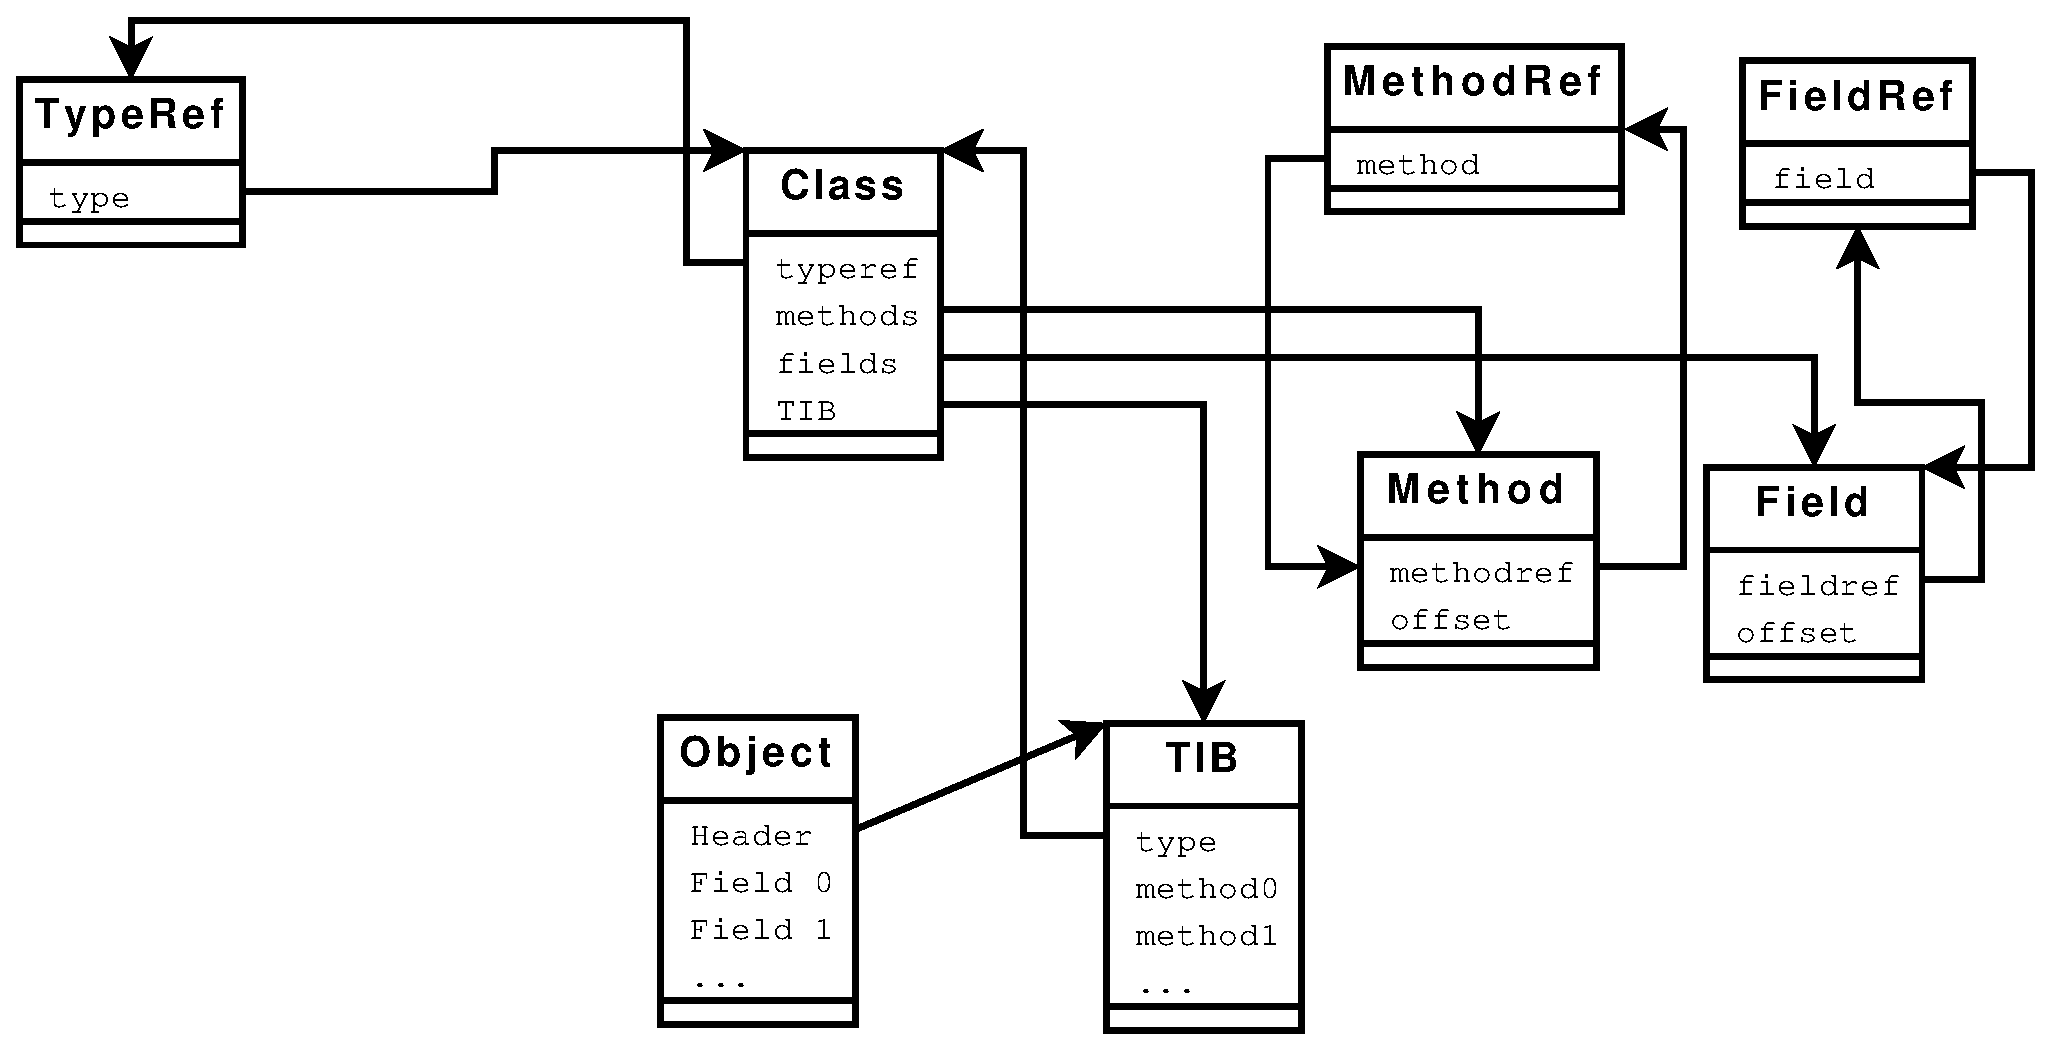
\includegraphics[width=0.84\paperwidth]{jvolve/vm-datastructures}
\end{center}
\end{frame}

\begin{frame}{VM Datastructures}%{A Sub-title is optional}
\begin{center}
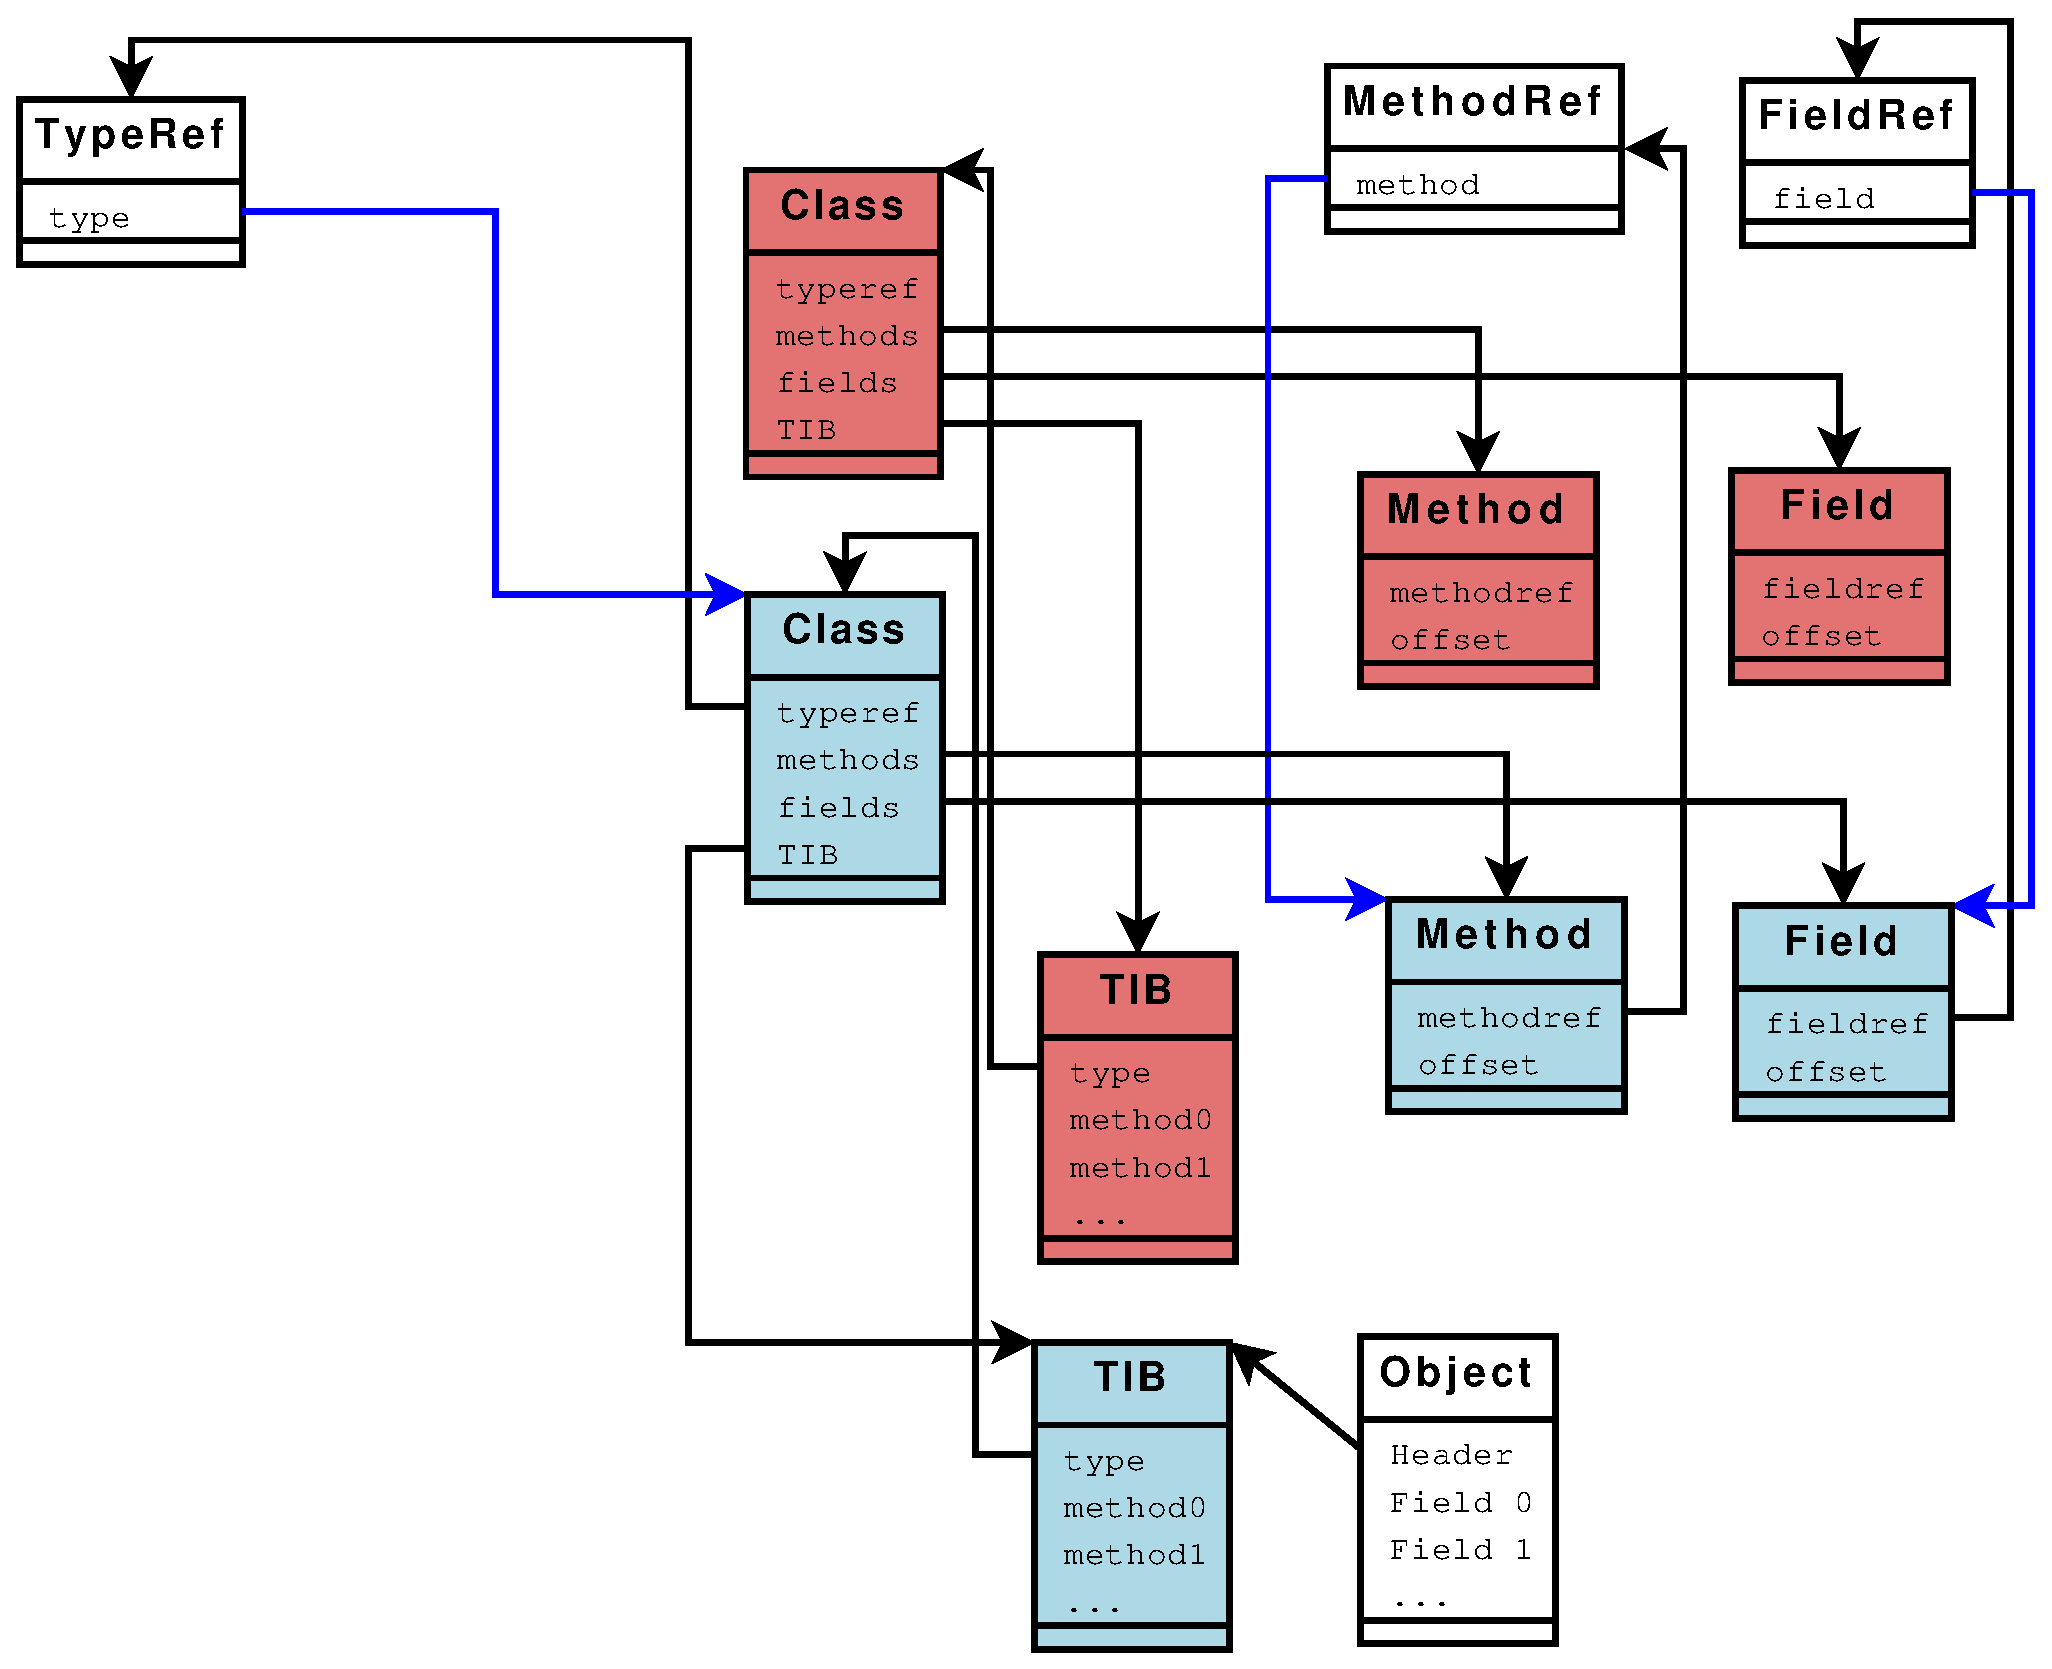
\includegraphics[width=0.84\paperwidth,height=0.7\paperheight]{jvolve/vm-datastructures-after-dsu}
\end{center}
\end{frame}

% \begin{frame}[fragile]{FXIME: Hierarchy}%{A Sub-title is optional}
% \begin{tikzpicture}
% \tikzstyle{every node}=[font=\scriptsize,circle,draw,minimum size=0.7cm]
% \tikzstyle{dsu node}=[every node,fill=structure.fg!50]
% \node at (0,0) (root) {A}
%   child {node {B}}
%   child {node[dsu node] {C}
%           child {node {D}}
%           child {node {E}}};
% \tikzstyle{level 1}=[sibling distance=3cm]
% \tikzstyle{level 2}=[sibling distance=2cm]
% \tikzstyle{level 3}=[sibling distance=1cm]
% \node at (6,0) {A}
%                       child {node {B}}
%                       child {node {C}
%                               child {node {D}}
%                               child {node {E}}}
%          child {node {Cx}
%                               child {node {Dx}}
%                               child {node {Ex}}}
%                      ;
% \end{tikzpicture}
% \end{frame}

\begin{frame}[t,fragile,label=transform]{Transforming objects}%{A Sub-title is optional}
\JvolveTimeLine{}{}{}{current}{}
\begin{itemize}
\item Built on top of a semi-space copying collector
\item Allocate additional space and run object transformers as part of the
      collector's visit
\end{itemize}
\end{frame}

\ifdraft{}{

%%%%%%%%%%%%%%%%%%%%%%%%%%%%%%%%%%%%%%%%%%%%%%%%%%%%%%%%%%%%%%%%%%%%%%%%
% Colors
\colorlet{black object color}{black!60}
\colorlet{grey object color}{black!20}
\colorlet{forwarding pointer color}{structure.fg!40}
\colorlet{dsu v0 color}{blue!60}
\colorlet{dsu v1 empty color}{blue!20}
\colorlet{dsu forwarding pointer color}{forwarding pointer color!50!dsu v0 color}
%%%%%%%%%%%%%%%%%%%%%%%%%%%%%%%%%%%%%%%%%%%%%%%%%%%%%%%%%%%%%%%%%%%%%%%%

%%%%%%%%%%%%%%%%%%%%%%%%%%%%%%%%%%%%%%%%%%%%%%%%%%%%%%%%%%%%%%%%%%%%%%%%
% Define the style for each field of the object
\newlength{\drawthickness}
\setlength{\drawthickness}{0.6pt}
\newlength{\fielddimension}
\setlength{\fielddimension}{5mm}
\tikzstyle{field}=[
    rectangle,
    draw=black,
    line width=\drawthickness,
    minimum width=\fielddimension,
    minimum height=\fielddimension,
    inner sep=0pt,
    font=\tiny,
]
\tikzstyle{new space grey field}=[field,fill=grey object color]
\tikzstyle{new space black field}=[field,fill=black object color]
\tikzstyle{dsu v0 field}=[field,fill=dsu v0 color]
\tikzstyle{dsu v1 empty field}=[field,fill=dsu v1 empty color]
%%%%%%%%%%%%%%%%%%%%%%%%%%%%%%%%%%%%%%%%%%%%%%%%%%%%%%%%%%%%%%%%%%%%%%%%

%%%%%%%%%%%%%%%%%%%%%%%%%%%%%%%%%%%%%%%%%%%%%%%%%%%%%%%%%%%%%%%%%%%%%%%%
% Define the style for each object
\tikzstyle{object}=[
    column sep=-\drawthickness,
    nodes=field,
    inner sep=0pt,
]
\tikzstyle{new space grey object}=[object,nodes=new space grey field]
\tikzstyle{new space black object}=[object,nodes=new space black field]
\tikzstyle{dsu v0 object}=[object,nodes=dsu v0 field]
\tikzstyle{dsu v1 empty object}=[object,nodes=dsu v1 empty field]
%%%%%%%%%%%%%%%%%%%%%%%%%%%%%%%%%%%%%%%%%%%%%%%%%%%%%%%%%%%%%%%%%%%%%%%%

%%%%%%%%%%%%%%%%%%%%%%%%%%%%%%%%%%%%%%%%%%%%%%%%%%%%%%%%%%%%%%%%%%%%%%%%
% Style for arrows
\tikzstyle{regular}=[-to,draw]
\tikzstyle{transparent}=[-to,draw=black!15!bg]
%%%%%%%%%%%%%%%%%%%%%%%%%%%%%%%%%%%%%%%%%%%%%%%%%%%%%%%%%%%%%%%%%%%%%%%%

%%%%%%%%%%%%%%%%%%%%%%%%%%%%%%%%%%%%%%%%%%%%%%%%%%%%%%%%%%%%%%%%%%%%%%%%
% Define a macro for creating an object with two fields
\newcommand{\twoFieldsObject}[3]{% name, position, object style
\matrix[#3,ampersand replacement=\&] (#1) at #2 {
  \node (#1 0) {}; \& \node (#1 1) {}; \\
};}
\newcommand{\fourFieldsObject}[3]{% name, position, object style
\matrix[#3,ampersand replacement=\&] (#1) at #2 {
  \node (#1 0) {}; \& \node (#1 1) {}; \& \node (#1 2) {}; \& \node (#1 3) {}; \\
};}


% Command to write a label next to an object
\newcommand{\labelObject}[4]{% label text, object name, label position, label anchor
\draw (#2.#3) node[anchor=#4,inner sep=0.5pt,font=\tiny] {#1};}
\newcommand{\oldSpaceLabelObject}[2]{% label text, object name
\labelObject{#1}{#2}{north west}{north east}}
\newcommand{\newSpaceLabelObject}[2]{% label text, object name
\labelObject{#1}{#2}{150}{south west}}

\newcommand{\oldSpaceObject}[3][object]{% object style, name, position
\twoFieldsObject{#2}{#3}{#1}\oldSpaceLabelObject{#2}{#2}}
\newcommand{\dsuOldSpaceVersionZeroObject}[2]{% name, location
\twoFieldsObject{#1}{#2}{dsu v0 object}\oldSpaceLabelObject{#1 $v_0$}{#1}}
\newcommand{\dsuOldSpaceVersionOneObject}[2]{% name, location
\fourFieldsObject{#1 v1}{#2}{dsu v1 empty object}\oldSpaceLabelObject{#1 $v_1$}{#1 v1}}

\newcommand{\newSpaceObject}[4][]{% extra name, name, position, object style
\twoFieldsObject{#2}{#3}{#4}\newSpaceLabelObject{#2#1}{#2}}
\newcommand{\newSpaceVersionOneEmptyObject}[2]{% name, position
\fourFieldsObject{#1 v1}{#2}{dsu v1 empty object}\labelObject{#1 $v_1$}{#1 v1}{165}{south west}}
\newcommand{\newSpaceGreyObject}[2]{% name, position
\newSpaceObject{#1}{#2}{new space grey object}}
\newcommand{\newSpaceBlackObject}[2]{% name, position
\newSpaceObject{#1}{#2}{new space black object}}
\newcommand{\dsuNewSpaceGreyObject}[2]{% name, position
\newSpaceObject[\ $v_0$]{#1}{#2}{new space grey object}}
\newcommand{\dsuNewSpaceBlackObject}[2]{% name, position
\newSpaceObject[\ $v_0$]{#1}{#2}{new space black object}}

\newcommand{\forwardingPointer}[1]{% name
\node[field,minimum width=2\fielddimension,fill=forwarding pointer color] at (#1.center) {#1'};
}
\newcommand{\dsuForwardingPointer}[1]{% name
\node[field,minimum width=2\fielddimension,fill=dsu forwarding pointer color] at (#1.center) {#1' $v_1$};
}
%%%%%%%%%%%%%%%%%%%%%%%%%%%%%%%%%%%%%%%%%%%%%%%%%%%%%%%%%%%%%%%%%%%%%%%%

%%%%%%%%%%%%%%%%%%%%%%%%%%%%%%%%%%%%%%%%%%%%%%%%%%%%%%%%%%%%%%%%%%%%%%%%
% Define coordinates of the various objects
\newcommand{\objectRoot}{(-3,0.8)}
\newcommand{\objectA}{(0,0)}
\newcommand{\objectB}{(-2,-1)}
\newcommand{\objectC}{(2,-1)}
\newcommand{\objectD}{(-3,-2)}
\newcommand{\objectE}{(-1,-2)}
\newcommand{\objectF}{(1,-2)}
\newcommand{\objectG}{(3,-2)}

\newcommand{\objectAprime}{(-3.5,0.25)}
\newcommand{\objectBprime}{(-2.5,0.25)}
\newcommand{\objectCprime}{(-1.5,0.25)}
\newcommand{\objectDprime}{(-0.5,0.25)}
\newcommand{\objectEprime}{(+0.5,0.25)}
\newcommand{\objectFprime}{(+1.5,0.25)}
\newcommand{\objectGprime}{(+2.5,0.25)}

% old space
\newcommand{\objectCVersionOne}{(2.5,0)}
\newcommand{\objectFVersionOne}{(1,-3)}
% new space
\newcommand{\objectCprimeVersionOne}{(-3,-1.75)}
\newcommand{\objectFprimeVersionOne}{(-0.75,-1.75)}
%%%%%%%%%%%%%%%%%%%%%%%%%%%%%%%%%%%%%%%%%%%%%%%%%%%%%%%%%%%%%%%%%%%%%%%%

% vim:tw=0:nospell


% The various steps of the animation are
% Slide 1: Show all objects
% Slide 2: A is copied
% Slide 3: A is scanned; B, C are copied
% Slide 4: A, B are scanned; C, D, E are copied
% Slide 5: A, B, C are scanned; D, E, F, G are copied
% Slide 6: A-D are scanned
% Slide 7: A-E are scanned
% Slide 8: A-F are scanned
% Slide 9: A-G are scanned
{
\begin{frame}[fragile]{Semi-space copying collector}%{A Sub-title is optional}
\setbeamercovered{invisible}
\begin{columns}[t]
\begin{column}[T]{0.67\paperwidth}
\begin{tikzpicture}
\begin{scope}
  % objects
  \uncover<1>{       \node[field] (root) at \objectRoot {root};                        }
  \uncover<2->{      \node[new space black field] (root) at \objectRoot {root};        }
                     \oldSpaceObject{A}{\objectA}
                     \oldSpaceObject{B}{\objectB}
                     \oldSpaceObject{C}{\objectC}
                     \oldSpaceObject{D}{\objectD}
                     \oldSpaceObject{E}{\objectE}
                     \oldSpaceObject{F}{\objectF}
                     \oldSpaceObject{G}{\objectG}
  % forwarding pointers
  \uncover<2->{      \forwardingPointer{A}                             }
  \uncover<3->{      \forwardingPointer{B}
                     \forwardingPointer{C}                             }
  \uncover<4->{      \forwardingPointer{D}
                     \forwardingPointer{E}                             }
  \uncover<5->{      \forwardingPointer{F}
                     \forwardingPointer{G}                             }
  % pointer arrows
  \uncover<1>   {    \path[regular]     (root.east)  to [out=330,in=120] (A.140)    ;          }
  \uncover<1>   {    \path[regular]     (A 0.center) to                (B.90)     ;            }
  \uncover<1>   {    \path[regular]     (A 1.center) to                (C.135)    ;            }
  \uncover<1-2> {    \path[regular]     (B 0.center) to                (D.135)    ;            }
  \uncover<1-2> {    \path[regular]     (B 1.center) to                (E.90)     ;            }
  \uncover<1-2> {    \path[regular]     (C 0.center) to                (F.135)    ;            }
  \uncover<1-2> {    \path[regular]     (C 1.center) to                (G.90)     ;            }
  \uncover<1-4> {    \path[regular]     (F 0.center) to                (A)        ;            }
                                                                      
  \uncover<2> {    \path[transparent]   (root.east)  to [out=0,in=120] (A.140)    ;            }
  \uncover<2> {    \path[transparent]   (A 0.center) to                (B.90)     ;            }
  \uncover<2> {    \path[transparent]   (A 1.center) to                (C.135)    ;            }
  \uncover<3> {    \path[transparent]   (B 0.center) to                (D.135)    ;            }
  \uncover<3> {    \path[transparent]   (B 1.center) to                (E.90)     ;            }
  \uncover<3> {    \path[transparent]   (C 0.center) to                (F.135)    ;            }
  \uncover<3> {    \path[transparent]   (C 1.center) to                (G.90)     ;            }
  \uncover<5> {    \path[transparent]   (F 0.center) to                (A)        ;            }

  \draw[draw,thin] (-4,-2.5) rectangle (4,0.5);
  \draw (4,0.5) node[anchor=north east,inner sep=1pt,font=\tiny] {FromSpace};

\end{scope}
\begin{scope}[yshift=-3.75cm]
  % objects
  \uncover<2>   {    \newSpaceGreyObject{A'}{\objectAprime}                          }
  \uncover<3->  {    \newSpaceBlackObject{A'}{\objectAprime}                         }

  \uncover<3>   {    \newSpaceGreyObject{B'}{\objectBprime}                          }
  \uncover<4->  {    \newSpaceBlackObject{B'}{\objectBprime}                         }

  \uncover<3-4> {    \newSpaceGreyObject{C'}{\objectCprime}                          }
  \uncover<5->  {    \newSpaceBlackObject{C'}{\objectCprime}                         }

  \uncover<4-5> {    \newSpaceGreyObject{D'}{\objectDprime}                          }
  \uncover<6->  {    \newSpaceBlackObject{D'}{\objectDprime}                         }

  \uncover<4-6> {    \newSpaceGreyObject{E'}{\objectEprime}                          }
  \uncover<7->  {    \newSpaceBlackObject{E'}{\objectEprime}                         }

  \uncover<5-7> {    \newSpaceGreyObject{F'}{\objectFprime}                          }
  \uncover<8->  {    \newSpaceBlackObject{F'}{\objectFprime}                         }

  \uncover<5-8> {    \newSpaceGreyObject{G'}{\objectGprime}                          }
  \uncover<9->  {    \newSpaceBlackObject{G'}{\objectGprime}                         }

  % pointer arrows
  \uncover<2->  {    \path[regular] (root.west)   to [out=220,in=95] (A'.north west);    }
  \uncover<2>   {    \path[regular] (A' 0.center) to [out=130,in=180] (B.west);
                     \path[regular] (A' 1.center) to [out=70,in=180]  (C.west);           }
  \uncover<3->  {    \path[regular] (A' 0.center) to [out=80,in=135]  (B'.150);          
                     \path[regular] (A' 1.center) to [out=70,in=150]  (C'.150);           }
                                                                                         
  \uncover<3>   {    \path[regular] (B' 0.center) to                  (D.south);         
                     \path[regular] (B' 1.center) to                  (E.south);          }
  \uncover<4->  {    \path[regular] (B' 0.center) to [out=300,in=240] (D'.215);          
                     \path[regular] (B' 1.center) to [out=330,in=240] (E'.215);           }
                                                                                         
  \uncover<3-4> {    \path[regular] (C' 0.center) to                  (F.south);         
                     \path[regular] (C' 1.center) to                  (G.south west);     }
  \uncover<5->  {    \path[regular] (C' 0.center) to [out=80,in=135]  (F'.150);          
                     \path[regular] (C' 1.center) to [out=70,in=150]  (G'.150);           }
                                                                                         
  \uncover<5-7> {    \path[regular] (F' 0.center) to [out=30,in=325]  (A);                }
  \uncover<8->  {    \path[regular] (F' 0.center) to [out=215,in=330] (A'.215);           }

  % transparent arrows
  \uncover<3>   {    \path[transparent] (A' 0.center) to [out=130,in=180] (B.west);
                     \path[transparent] (A' 1.center) to [out=70,in=180]  (C.west);       }

  \uncover<4>   {    \path[transparent] (B' 0.center) to                  (D.south);
                     \path[transparent] (B' 1.center) to                  (E.south);      }

  \uncover<5>   {    \path[transparent] (C' 0.center) to                  (F.south);
                     \path[transparent] (C' 1.center) to                  (G.south west); }

  \uncover<8>   {    \path[transparent] (F' 0.center) to [out=30,in=325]  (A);            }
  

  \draw[draw,thin] (-4,-2) rectangle (4,0.5);
  \draw (4,-2) node[anchor=south east,inner sep=1pt,font=\tiny] {ToSpace};
\end{scope}
\end{tikzpicture}
\end{column}
\begin{column}[T]{0.25\paperwidth}
\begin{block}{}
\begin{tikzpicture}
\tikzstyle{column 2}=[anchor=west]
\matrix [row sep=0.5ex] {
\node[new space grey field] {};                & \node {\tiny Visited}; \\
\node[new space black field] {};               & \node {\tiny All children visited}; \\
\node[field,fill=forwarding pointer color] {}; & \node {\tiny Forwarding pointer}; \\
};
\end{tikzpicture}
\end{block}

\begin{block}{}
\begin{scriptsize}
\only<1>{
The heap is divided into two spaces. Only one space is used by the
application. The garbage collector copies objects from \emph{FromSpace} to
\emph{ToSpace}.
}
\only<2>{
GC copies A to \emph{ToSpace}, leaves a forwarding pointer pointing to the
new copy A'.
}
\only<3>{
GC scans A'. The objects pointed to by A' (B and C) are copied to
\emph{ToSpace}. A's fields point to the copied objects.
}
\only<4>{
Next, the GC scans B', and copies objects D and E.
}
\only<5-7>{
Similarly for C'\uncover<6-7>{, D'}\uncover<7>{, and E.}
}
\only<8>{
When scanning F', the first field points to A in \emph{FromSpace}, which is a
forwarding pointer. After the scan, this field points to A'.
}
\only<9>{
All objects in \emph{ToSpace} are scanned. All reachable/live objects are now
in \emph{ToSpace}.
}
\end{scriptsize}
\end{block}
\end{column}
\end{columns}
\end{frame}
}

% vim:tw=0:nospell

}

\begin{frame}[t,fragile]{\DSU{} Garbage collector}%{A Sub-title is optional}
\JvolveTimeLine{}{}{}{current}{}
\begin{itemize}
\item Identical to Semispace for ``regular'' objects
\item For objects to be transformed
  \begin{itemize}
  \item Copy the object to ToSpace (like Semispace)
  \item Also, allocate an empty object in ToSpace for the new version
  \end{itemize}
\item Forwarding pointers point to the ``new version'' object
\item No field can point to an ``old version'' object
\end{itemize}
\end{frame}

\ifdraft{}{

%%%%%%%%%%%%%%%%%%%%%%%%%%%%%%%%%%%%%%%%%%%%%%%%%%%%%%%%%%%%%%%%%%%%%%%%
% Now, we show semispace with objects being updated.
%%%%%%%%%%%%%%%%%%%%%%%%%%%%%%%%%%%%%%%%%%%%%%%%%%%%%%%%%%%%%%%%%%%%%%%%
{
\begin{frame}[fragile]{\DSU{} garbage collector}%{A Sub-title is optional}
\setbeamercovered{invisible}
\begin{columns}[t]
\begin{column}[T]{0.67\paperwidth}
\begin{tikzpicture}
\begin{scope}
  % objects
  \uncover<1>{       \node[field] (root) at \objectRoot {root};                        }
  \uncover<2->{      \node[new space black field] (root) at \objectRoot {root};        }
                     \oldSpaceObject{A}{\objectA}
                     \oldSpaceObject{B}{\objectB}
                     \oldSpaceObject[dsu v0 object]{C}{\objectC}
                     \oldSpaceObject{D}{\objectD}
                     \oldSpaceObject{E}{\objectE}
                     \oldSpaceObject[dsu v0 object]{F}{\objectF}
                     \oldSpaceObject{G}{\objectG}
  % forwarding pointers
  \uncover<2->{      \forwardingPointer{A}                             }
  \uncover<3->{      \forwardingPointer{B}
                     \dsuForwardingPointer{C}                          }
  \uncover<4->{      \forwardingPointer{D}
                     \forwardingPointer{E}                             }
  \uncover<5->{      \dsuForwardingPointer{F}
                     \forwardingPointer{G}                             }
  % pointer arrows
  \uncover<1>   {    \path[regular]     (root.east)  to [out=330,in=120] (A.140)    ;          }
  \uncover<1>   {    \path[regular]     (A 0.center) to                (B.90)     ;            }
  \uncover<1>   {    \path[regular]     (A 1.center) to                (C.135)    ;            }
  \uncover<1-2> {    \path[regular]     (B 0.center) to                (D.135)    ;            }
  \uncover<1-2> {    \path[regular]     (B 1.center) to                (E.90)     ;            }
  \uncover<1-2> {    \path[regular]     (C 0.center) to                (F.135)    ;            }
  \uncover<1-2> {    \path[regular]     (C 1.center) to                (G.90)     ;            }
  \uncover<1-4> {    \path[regular]     (F 0.center) to                (A)        ;            }
                                                                      
  \uncover<2> {    \path[transparent]   (root.east)  to [out=0,in=120] (A.140)    ;            }
  \uncover<2> {    \path[transparent]   (A 0.center) to                (B.90)     ;            }
  \uncover<2> {    \path[transparent]   (A 1.center) to                (C.135)    ;            }
  \uncover<3> {    \path[transparent]   (B 0.center) to                (D.135)    ;            }
  \uncover<3> {    \path[transparent]   (B 1.center) to                (E.90)     ;            }
  \uncover<3> {    \path[transparent]   (C 0.center) to                (F.135)    ;            }
  \uncover<3> {    \path[transparent]   (C 1.center) to                (G.90)     ;            }
  \uncover<5> {    \path[transparent]   (F 0.center) to                (A)        ;            }

  \draw[draw,thin] (-4,-2.5) rectangle (4,0.5);
  \draw (4,0.5) node[anchor=north east,inner sep=1pt,font=\tiny] {FromSpace};

\end{scope}
\begin{scope}[yshift=-3.75cm]
  % objects
  \uncover<2>   {    \newSpaceGreyObject{A'}{\objectAprime}                          }
  \uncover<3->  {    \newSpaceBlackObject{A'}{\objectAprime}                         }

  \uncover<3>   {    \newSpaceGreyObject{B'}{\objectBprime}                          }
  \uncover<4->  {    \newSpaceBlackObject{B'}{\objectBprime}                         }

  \uncover<3-4> {    \dsuNewSpaceGreyObject{C'}{\objectCprime}                       }
  \uncover<5-10>{    \dsuNewSpaceBlackObject{C'}{\objectCprime}                      }
  \uncover<3->  {    \newSpaceVersionOneEmptyObject{C'}{\objectCprimeVersionOne}     }

  \uncover<4-5> {    \newSpaceGreyObject{D'}{\objectDprime}                          }
  \uncover<6->  {    \newSpaceBlackObject{D'}{\objectDprime}                         }

  \uncover<4-6> {    \newSpaceGreyObject{E'}{\objectEprime}                          }
  \uncover<7->  {    \newSpaceBlackObject{E'}{\objectEprime}                         }

  \uncover<5-7> {    \dsuNewSpaceGreyObject{F'}{\objectFprime}                       }
  \uncover<8-10>{    \dsuNewSpaceBlackObject{F'}{\objectFprime}                      }
  \uncover<5->  {    \newSpaceVersionOneEmptyObject{F'}{\objectFprimeVersionOne}     }

  \uncover<5-8> {    \newSpaceGreyObject{G'}{\objectGprime}                          }
  \uncover<9->  {    \newSpaceBlackObject{G'}{\objectGprime}                         }

  % pointer arrows
  \uncover<2->  {    \path[regular] (root.west)   to [out=220,in=95] (A'.north west);    }
  \uncover<2>   {    \path[regular] (A' 0.center) to [out=130,in=180] (B.west);
                     \path[regular] (A' 1.center) to [out=70,in=180]  (C.west);           }
  \uncover<3->  {    \path[regular] (A' 0.center) to [out=80,in=135]  (B'.150);          
                     \path[regular] (A' 1.center) to [out=270,in=110] (C' v1.north west); }
                                                                                         
  \uncover<3>   {    \path[regular] (B' 0.center) to                  (D.south);         
                     \path[regular] (B' 1.center) to                  (E.south);          }
  \uncover<4->  {    \path[regular] (B' 0.center) to [out=300,in=240] (D'.215);          
                     \path[regular] (B' 1.center) to [out=330,in=240] (E'.215);           }
                                                                                         
  \uncover<3-4> {    \path[regular] (C' 0.center) to                  (F.south);         
                     \path[regular] (C' 1.center) to                  (G.south west);     }
  \uncover<5-10>{    \path[regular] (C' 0.center) to [out=255,in=105]  (F' v1.north west);          
                     \path[regular] (C' 1.center) to [out=70,in=150]  (G'.150);           }
                                                                                         
  \uncover<5-7> {    \path[regular] (F' 0.center) to [out=30,in=325]  (A);                }
  \uncover<8-10>{    \path[regular] (F' 0.center) to [out=215,in=330] (A'.215);           }

  % transparent arrows
  \uncover<3>   {    \path[transparent] (A' 0.center) to [out=130,in=180] (B.west);
                     \path[transparent] (A' 1.center) to [out=70,in=180]  (C.west);       }

  \uncover<4>   {    \path[transparent] (B' 0.center) to                  (D.south);
                     \path[transparent] (B' 1.center) to                  (E.south);      }

  \uncover<5>   {    \path[transparent] (C' 0.center) to                  (F.south);
                     \path[transparent] (C' 1.center) to                  (G.south west); }

  \uncover<8>   {    \path[transparent] (F' 0.center) to [out=30,in=325]  (A);            }

  % v1 arrows
  \uncover<10-> {    \path[regular] (C' v1 0.center) to [out=30,in=120]   (F' v1.north west);
                     \path[regular] (C' v1 1.center) to                   (G'.210);          
                     \path[regular] (F' v1 0.center) to [out=180,in=315]  (A'.215);
                }
  

  \draw[draw,thin] (-4,-2) rectangle (4,0.5);
  \draw (4,-2) node[anchor=south east,inner sep=1pt,font=\tiny] {ToSpace};
\end{scope}
\end{tikzpicture}
\end{column}
\begin{column}[T]{0.25\paperwidth}
\begin{block}{}
\begin{tikzpicture}
\tikzstyle{column 2}=[anchor=west]
\matrix [row sep=0.5ex] {
\node[dsu v0 field] {};          & \node {\tiny To be transformed}; \\
\node[dsu v1 empty field] {};    & \node {\tiny $v_1$ object}; \\
};
\end{tikzpicture}
\end{block}

\begin{block}{}
\begin{footnotesize}
\only<1>{
The same heap as before. Objects to be transformed are highlighted.
}
\only<2>{
Copy A.
}
\only<3>{
Scan A'. Copy B and C. In addition an empty object C'$v_1$ is allocated.
\alert{A' points to this copy and not the old one.}
}
\only<4>{
Scan B'.
}
\only<5>{
Scan C'.
}
\only<6>{
Scan D'.
}
\only<7>{
Scan E'.
}
\only<8>{
Scan F'.
}
\only<9>{
GC is now complete. No field can point to C'$v_0$ or F'$v_0$. Pointers to C and
F point to $v_1$ (empty) objects. \texttt{memcpy(v\_1, v\_0);} will give us a valid
heap.}
\only<10>{
Setting fields of C'$v_1$ and F'$v_1$.
}
\only<11>{
C'$v_0$ and F'$v_0$ can be reclaimed.
}
\end{footnotesize}
\end{block}
\end{column}
\end{columns}
\end{frame}
}

% vim:tw=0:nospell

{
\begin{frame}[fragile]{\DSU{} Garbage collector}%{A Sub-title is optional}
\setbeamercovered{invisible}
\begin{center}
\begin{tikzpicture}
  % objects
                  \node[field] (root) at \objectRoot {root};
                  \oldSpaceObject{A}{\objectA}
                  \oldSpaceObject{B}{\objectB}
\uncover<-1>{     \dsuOldSpaceVersionZeroObject{C}{\objectC}                  }
                  \oldSpaceObject{D}{\objectD}
                  \oldSpaceObject{E}{\objectE}
\uncover<-1>{     \dsuOldSpaceVersionZeroObject{F}{\objectF}                  }
                  \oldSpaceObject{G}{\objectG}

                  \dsuOldSpaceVersionOneObject{C}{\objectCVersionOne}
                  \dsuOldSpaceVersionOneObject{F}{\objectFVersionOne}

                  % pointer arrows
                  \path[regular]     (root.east)  to [out=330,in=120]     (A.140);
                  \path[regular]     (A 0.center) to                      (B.90);
                  \path[regular]     (A 1.center) to                      (C v1.190);
                  \path[regular]     (B 0.center) to                      (D.135);
                  \path[regular]     (B 1.center) to                      (E.90);
\uncover<-1>{     \path[regular]     (C 0.center) to [out=180,in=90]      (F v1.north west);
                  \path[regular]     (C 1.center) to                      (G.90);
                  \path[regular]     (F 0.center) to                      (A);                       }

\uncover<2-2>{    \path[regular]     (C v1 0.center) to [out=180,in=120]  (F v1.north west);
                  \path[regular]     (C v1 1.center) to                   (G.60);
                  \path[regular]     (F v1 0.center) to                   (A);                       }

  \draw[draw,thin] (-4,-3.5) rectangle (4,0.5);
\end{tikzpicture}
\begin{block}{}
\begin{itemize}
\item No field can point to an ``old version'' object
\item ``new version'' objects are all empty
\item Run transformation functions after GC to fill in fields
\end{itemize}
\end{block}
\end{center}
\end{frame}
}

% vim:tw=0:nospell

{
\begin{frame}[fragile]{Revisiting transformation functions}%{A Sub-title is optional}
\setbeamercovered{invisible}
\begin{center}
\begin{tikzpicture}
  % objects
  \node[field] (root) at \objectRoot {root};
  \oldSpaceObject{A}{\objectA}
  \oldSpaceObject{B}{\objectB}
  \dsuOldSpaceVersionZeroObject{C}{\objectC}
  \oldSpaceObject{D}{\objectD}
  \oldSpaceObject{E}{\objectE}
  \dsuOldSpaceVersionZeroObject{F}{\objectF}
  \oldSpaceObject{G}{\objectG}
  \dsuOldSpaceVersionOneObject{C}{\objectCVersionOne}
  \dsuOldSpaceVersionOneObject{F}{\objectFVersionOne}

  % pointer arrows
  \path[regular]     (root.east)  to [out=330,in=120]     (A.140);
  \path[regular]     (A 0.center) to                      (B.90);
  \path[regular]     (A 1.center) to                      (C v1.190);
  \path[regular]     (B 0.center) to                      (D.135);
  \path[regular]     (B 1.center) to                      (E.90);
  \path[regular]     (C 0.center) to [out=180,in=90]      (F v1.north west);
  \path[regular]     (C 1.center) to                      (G.90);
  \path[regular]     (F 0.center) to                      (A);

  \draw[draw,thin] (-4,-3.5) rectangle (4,0.5);
\end{tikzpicture}
\begin{block}{We have an ordering problem}
\texttt{(C $v_0$).field0.field0} might be uninitialized
\end{block}
\end{center}
\end{frame}
}

% vim:tw=0:nospell

}

\begin{frame}[t,fragile]{Revisiting transformation functions}%{A Sub-title is optional}
\JvolveTimeLine{}{}{}{current}{}
Solutions to the ordering problem \\
\begin{itemize}
\item Programmer can invoke a VM function that will transform objects on
demand. Moves burden of safety to the programmer
\item<2-> Insert read barrier code to perform this check when compiling the
transformation function
\item<2-> Perform some static analysis to determine an order to queue
objects
% \item<2-> Change the collector's traversal to reverse-postorder
\end{itemize}
\end{frame}

\begin{frame}{Proposed work}%{A Sub-title is optional}
\begin{itemize}
\item Improving flexibility: On-stack replacement (OSR) support
\item Improving efficiency: Concurrent collector support
\end{itemize}
\end{frame}

\begin{frame}[t,fragile]{Extending On-stack replacement (OSR)}%{A Sub-title is optional}
\JvolveTimeLine{}{current}{}{}{current}
\begin{itemize}
\item Some updates cannot be performed because the VM does not reach a DSU
      safe point
\item \JikesRVM{} employs OSR to promote long running methods for
      optimization
      \begin{itemize}
      \item Extract compiler-independent state from an activation record
      \item Generate a \emph{specialized prologue} that sets up local
            variables
      \item Jump to corresponding program counter in optimized code
      \end{itemize}
\item We can utilize this functionality taking into account old and new
versions
\end{itemize}
\end{frame}

\begin{frame}[t,fragile]{OSR issues}%{A Sub-title is optional}
\JvolveTimeLine{}{current}{}{}{current}
\begin{itemize}
\item What types of updates can benefit from OSR?
\item How does OSR know where to resume execution?
\item What about new local variables and those that need to be transformed?
\item OSR in \JikesRVM{} can only replace the topmost method on stack.
  \begin{itemize}
  \item Implement ``return barriers''
  \item Overwrite return addresses and jump to VM code that will perform
        OSR for the current top method
  \item Some methods might be long running and always belong to some old
        version
  \end{itemize}
\end{itemize}
\end{frame}

\begin{frame}[t,fragile]{\DSU{} efficiency}%{A Sub-title is optional}
\JvolveTimeLine{}{}{}{current}{}
\begin{itemize}
\item \DSU{} requires a stop-the-world full-heap GC
\item Update time is dominated by GC time
\item Real-time and highly available applications use a concurrent GC
\end{itemize}
\end{frame}

\begin{frame}[t,fragile]{\DSU{} with a concurrent collector}%{A Sub-title is optional}
\JvolveTimeLine{}{}{}{current}{}
\begin{itemize}
\item Application and collector run concurrently
\item Guard application from accessing an object of the old version
\item Collectors already use read/write barriers to guard the application
      from disrupting the tricolor abstraction. Piggyback on these
      barriers for DSU
\item What is the additional overhead?
\item How flexible can object transformers be?
\end{itemize}
\end{frame}

% Section 4: Experience & Performance
%   Describe the applications we could update
%   Updates we couldn't support
%   Measurements
%     How long until updates take effect in certain circumstances
%       (i.e., how onerous is our timing-based safety condition?)
%     How long do updates take
%       (i.e., what's the cost of a full GC?)
%     What's the impact on performance?
%       (i.e., is there any impact to performance after an update is done?)
%       (i.e., how much is end-to-end application performance hampered by an
%         update?  E.g., to web connections time out, etc.?)
%     We're doing micro- and macro-benchmarks, right?  What are they?

\section{Experience}
\label{sec:experience}

\suriya{Changes to experience section marked up by Kathryn have to
incorporated. This involves running additional experiments as well. All
other sections done.}

To evaluate \DSU, we used it to update three open-source servers written
in Java: the Jetty webserver\footnote{\url{http://www.mortbay.org}},
JavaEmailServer,\footnote{\url{http://www.ericdaugherty.com/java/mailserver}}
an SMTP and POP e-mail server, and CrossFTP server\footnote{\url{http://www.crossftp.com/}}.
These programs belong to a class that
should benefit from DSU because they typically run continuously. DSU
would enable deployments to incorporate bug fixes or add new features
without having to halt currently-running sessions.  We explored
updates corresponding to releases made over roughly a year and a half
of each program's lifetime.  Of 22 updates we considered, \DSU{} could
support 20 of them---the two updates we could not apply changed
classes with infinitely-running methods, and thus no safe point could
be reached.  To our knowledge, no existing DSU system
for Java could support these updates, and furthermore previous systems
would support only 9 of 22 updates.  \DSU{} is the first DSU system for Java
that has been shown to support changes to realistic programs as they
occur in practice over a long period.  The remainder of this section
describes this experience.

\subsection{Jetty webserver}
\label{subsec:jetty}

Jetty is a widely-used webserver written in Java, in development since
1995.  It supports static and dynamic content and can be embedded
within other Java applications.  The \JikesRVM{} is not able to run the
most recent versions of Jetty (6.x), therefore we considered 11
versions, consisting of 5.1.0 through 5.1.10 (the last one prior to
version 6).  Version 5.1.10 contains 317 classes and about 45000 lines
of code.  Table~\ref{tab:jetty-changes} shows a summary of the changes
in each update.  Each row tabulates the changes relative
to the prior version. For the column listing changed methods, the
notation $x/y$ indicates that $x+y$ methods were changed, where $x$
changed in body only, and $y$ changed their type signature as well.
For dynamic updating systems that only support changes to method
bodies, only the first and last three of the ten updates could be
expressed, since the remainder either change method signatures
and/or add or delete fields.

% \DSU{} was able to successfully update from
% each version to the next for all versions except 5.1.3 and 5.1.5.
% Both of these updates were precluded by our update preparation tool
% because it fails to properly identify changes to anonymous inner
% classes.  We believe this limitation is the only one needed to support
% these updates and we plan to have this functionality for the final
% paper.

\newcommand{\ChangedClassesColumn}{third}
\begin{table}
\begin{footnotesize}
\begin{center}
\begin{tabular}{|l||c||c|c|c|c|c|c|} \hline
Ver.    & \#      & \multicolumn{6}{c|}{\# changed} \\
        & classes & classes & \multicolumn{3}{c|}{methods} & \multicolumn{2}{c|}{fields} \\
        & added   &         & add & del & chg              & add & del \\ \hline \hline
5.1.1   & 0       & 14      & 4   & 1   & 38/0             & 0   & 0   \\
5.1.2   & 1       & 5       & 0   & 0   & 12/1             & 0   & 0   \\
5.1.3   & 3       & 15      & 19  & 2   & 59/0             & 10  & 1   \\
5.1.4   & 0       & 6       & 0   & 4   & 9/6              & 0   & 2   \\
5.1.5   & 0       & 54      & 21  & 4   & 112/8            & 5   & 0   \\
5.1.6   & 0       & 4       & 0   & 0   & 20/0             & 5   & 6   \\
5.1.7   & 0       & 7       & 8   & 0   & 11/2             & 9   & 3   \\
5.1.8   & 0       & 1       & 0   & 0   & 1/0              & 0   & 0   \\
5.1.9   & 0       & 1       & 0   & 0   & 1/0              & 0   & 0   \\
5.1.10  & 0       & 4       & 0   & 0   & 4/0              & 0   & 0   \\ \hline
\end{tabular}
\end{center}
\end{footnotesize}
\caption{Summary of updates to Jetty}
\label{tab:jetty-changes}
\end{table}

With \DSU{} we were able to successfully write dynamic updates to all
versions of Jetty we examined.  However, we could not apply an update
to version 5.1.3 because \DSU{} was never able to reach a safe point.
To understand why, we instrumented the VM to emit information about
restricted method set and, if a safe point cannot be reached, which
restricted method was active.  For each version, starting at 5.1.0, we
ran Jetty under full load.  After 30 seconds we tried to apply the
update to the next version; if a safe point could not be immediately
reached, we deemed the attempt as failed (i.e., we did not retry).  
The results are presented in
Table~\ref{tab:inlining}.  Column 2 shows the number of times (out of
five such runs) the application reached a safe point.  The methods
whose presence on a thread stack precluded the application from
reaching a safe point are mentioned below the table.  For the update
to 5.1.3, the offending method was always
active (it contained an infinite loop).  The other updates either
always succeeded, or did most of the time, implying that with retries
they could be applied fairly quickly.

Column 3 contains the total number
of methods in the program at runtime, where the number in parentheses is the
number of these the compiler inlined when using aggressive optimization
(which provides an upper bound on the effect of inlining in reaching a
safe point).  The next group of columns contains the restricted method
set. Each column in the group specifies the number of methods loaded at
run time by the VM, followed by the total number of methods in that
category in the program. The first column in this group is the number of methods in
classes involved in a class update. Recall that when a class is updated, say by adding
a field, all its methods are considered restricted. The second column in this group is the number of methods whose
bodies are updated, the third is the number of methods
indirectly updated, and the fourth sums these, with the number of the
total that were inlined written in parentheses. % The first and second
% columns in this group together constitute all the methods of classes that
% were changed, as enumerated in the \ChangedClassesColumn{} column in table~\ref{tab:jetty-changes}.
The final column is
the total number of methods in the restricted set; it differs from the
first number in the fourth column by the number of (transitively)
inlined callers of the restricted methods that were not already
restricted.

The table shows that both indirect method calls and inlining 
significantly add to the size of the restricted set,
though inlining is small by comparison because all callers of an
updated class's methods are \emph{already} included in the indirect
set, so inlining these methods adds no further restriction.
Interestingly, having a greater number of restricted methods overall
does not necessarily reduce the likelihood that an update will take
effect; rather, it depends on the frequency with which methods in this
set are on the stack.
% In the
% case of Jetty, none of this had any impact on the update failing:
% version 5.1.3 changed the bodies of the infinite loops of active
% threads' \texttt{run} methods, and thus reaching a safe point was
% not possible.  
% Future support 
% for updates based on on-stack replacement may alleviate this problem.

\begin{table*}
\begin{small}
\begin{center}
\begin{tabular}{|c|c|r|rrrr|r|} \hline
Upd.    &                   & Number of  & \multicolumn{4}{c|}{\# methods not allowed on stack, due to}                 & Number of \\
to      & Reached           & methods at & \emph{class}   & \emph{method body} & \emph{indirect method}  &              & restricted \\
ver.    & safe point?       & runtime    & \emph{updates} & \emph{updates}     & \emph{updates}          & Total        & methods   \\ \hline \hline
5.1.1   &  always           & 1378 (376) & 26/49          & 7/12               & 20/29                   & 53/90  (17)  & 67        \\
5.1.2   &  4/5$^\dagger$    & 1374 (375) & 25/25          & 3/5                & 35/43                   & 63/73  (35)  & 67        \\
5.1.3   &  0/5$^*$          & 1374 (375) & 326/382        & 4/6                & 42/45                   & 370/433 (97) & 373       \\
5.1.4   &  always           & 1384 (374) & 82/82          & 5/6                & 15/16                   & 101/104 (24) & 101       \\
5.1.5   &  always           & 1380 (372) & 14/80          & 39/60              & 13/15                   & 62/155 (17)  & 62        \\
5.1.6   &  3/5$^\dagger$    & 1394 (378) & 203/219        & 3/3                & 16/19                   & 222/241 (40) & 223       \\
5.1.7   &  always           & 1394 (380) & 186/187        & 1/2                & 53/69                   & 239/258 (74) & 243       \\
5.1.8   &  always           & 1402 (379) & 0/0            & 1/1                & 0/0                     & 1/1   (1)    & 1         \\
5.1.9   &  always           & 1402 (379) & 0/0            & 0/1                & 0/0                     & 0/1   (0)    & 0         \\
5.1.10  &  always           & 1402 (379) & 0/0            & 4/5                & 0/0                     & 4/5   (2)    & 6         \\ \hline
\end{tabular}
\end{center}
\begin{tabular}{l}
$^\dagger$Restricted method \texttt{HttpConnection.handleNext()} was
active \\
$^*$Restricted method \texttt{ThreadedServer.acceptSocket()} was
(always) active
\end{tabular}
\end{small}
\vspace{1ex}
\caption{Impact of safe point restrictions on updates to Jetty}
\label{tab:inlining}
\end{table*}

\subsection{JavaEmailServer}
\label{subsec:jes}

For JavaEmailServer we looked at 10 versions---1.2.1 through
1.4---spanning a duration of about two years.  The final version of
the code consists of 20 classes and about 5000 lines of code.
Table~\ref{tab:jes-changes} shows the summary of changes for each new
version. Approaches that only support updates to method bodies will be able
to handle only four of the nine updates we considered. We
could successfully construct updates for all versions we examined, and
we could successfully apply all of them but the update to version 1.3.  This
update reworked the configuration framework of the server, among other
things removing a GUI tool for user administration and added several
new classes to implement a file-based system.  As a result, many of
the classes were modified to point to a new configuration object,
among these threads with infinite processing loops (e.g., to accept
POP and SMTP requests).  Because these classes are always active, the
safety condition can never be met and thus the update cannot be
applied.

In addition, for the update from 1.3 to 1.3.1, the processing loop of
one class was \emph{indirectly} updated, and this initially precluded
the update from taking place.  To remedy this problem, we manually
extracted the body of the loop and made it a separate function,
essentially a manual application of the ``loop extraction''
transformation used in other work~\cite{neamtiu06dsu}.  However, even
in this case the update would only take effect if the server was idle;
a similar situation occurred for the update to version 1.3.3.  We
could avoid this transformation and the need for idleness by using a
limited form of on-stack replacement 
(OSR) in combination with stack barriers, as mentioned in
Section~\ref{sec:safe}.  Note that loop extraction would 
not help for our other problematic updates because it was the
\texttt{run} methods themselves whose code was changed, and not some
method that they call.

%% This application was defensively written in terms of handling exceptions.
%% There were several top-level exception handlers that kept the application
%% going even if a particular piece of code or a particular thread threw an
%% exception. The application relied on very little soft persistent state.
%% State about user accounts, mail queue were maintained in disk outside the
%% application in configuration files and mailbox files. These were
%% periodically watched for changes. This made updates also easier. Any
%% incorrect update would respawn a new thread, and have persistent state
%% (since it is outside the program).

\begin{table}
\begin{footnotesize}
\begin{center}
\begin{tabular}{|l||c|c||c|c|c|c|c|c|} \hline
Ver.   & \multicolumn{2}{c||}{\# classes} &    \multicolumn{6}{c|}{\# changed} \\
       & add & del & classes & \multicolumn{3}{c|}{methods} & \multicolumn{2}{c|}{fields} \\
       &     &     &         & add & del & chg   & add & del \\ \hline \hline
1.2.2  & 0   & 0   & 3       & 0   & 0   & 3/0   & 0   & 0   \\
1.2.3  & 0   & 0   & 7       & 0   & 0   & 14/2  & 12  & 0   \\
1.2.4  & 0   & 0   & 2       & 0   & 0   & 4/0   & 0   & 0   \\
1.3    & 4   & 9   & 2       & 11  & 3   & 6/9   & 12  & 5   \\
1.3.1  & 0   & 0   & 2       & 0   & 0   & 4/0   & 0   & 0   \\
1.3.2  & 0   & 0   & 8       & 4   & 2   & 4/2   & 3   & 1   \\
1.3.3  & 0   & 0   & 4       & 0   & 0   & 3/0   & 0   & 0   \\
1.3.4  & 0   & 0   & 6       & 2   & 0   & 6/0   & 2   & 0   \\
1.4    & 0   & 0   & 7       & 6   & 1   & 4/1   & 6   & 0   \\ \hline
\end{tabular}
\end{center}
\end{footnotesize}
\caption{Summary of updates to JavaEmailServer}
\label{tab:jes-changes}
\end{table}

% 
% Summary of JES safe-point-convergence
% update to v1.3 does not happen even when idle.
% update to 1.3.1 and update to 1.3.3 
% happens when idle, but never happens with load
% In both cases the offending function is SMTPProcessor.handleCommands()
% All other updates happened all the time.
%

\subsection{CrossFTP server}
\label{subsec:crossftp}
CrossFTP server is an easily configurable, secure-enabled FTP server.
CrossFTP allows simple configuration through a GUI and more advanced
customization using configuration files. We did not use the GUI interface
and therefore do not consider changes to that part of the program.  We
looked at 4 versions --- 1.05 through 1.08 --- spanning a duration of more
than a year. Version 1.08 contains about 18000 lines of code spread across
161 classes. We could successfully handle all three updates to this
application, though one update would apply only rarely under
load. Note that since all updates either add or delete fields, simple 
method body updating support on its own would be insufficient.

% \begin{table}
% \begin{scriptsize}
% \begin{center}
% \begin{tabular}{|l||c|c||c|c|c|c|c|c||c|} \hline
% Ver.   & \multicolumn{2}{c||}{\# classes} &    \multicolumn{6}{c||}{\# changed}            & Reached \\
%        & add & del & classes & \multicolumn{3}{c|}{methods} & \multicolumn{2}{c||}{fields} & safe    \\
%        &     &     &         & add & del & chg   & add & del                               & point?  \\ \hline \hline
% 1.06   & 4   & 1   & 1       & 0   & 0   & 3/0   & 1   & 0                                 & always \\
% 1.07   & 0   & 0   & 3       & 4   & 0   & 14/0  & 5   & 0                                 & 3/5$^1$ \\
% 1.08   & 0   & 1   & 3       & 2   & 0   & 10/0  & 0   & 2                                 & 1/5$^2$ \\ \hline
% \end{tabular}
% \end{center}
% \begin{tabular}{l}
% $^1$Restricted method \texttt{RequestHandler.run()} was active \\
% $^2$Restricted methods \texttt{FTPWriter.send()}, \texttt{RequestHandler.run()} were active \\
% \end{tabular}
% \end{scriptsize}
% \caption{Summary of updates to CrossFTP server}
% \label{tab:crossftp-changes}
% \end{table}

\begin{table}
\begin{footnotesize}
\begin{center}
\begin{tabular}{|l||c|c||c|c|c|c|c|c|} \hline
Ver.   & \multicolumn{2}{c||}{\# classes} &    \multicolumn{6}{c|}{\# changed}             \\
       & add & del & classes & \multicolumn{3}{c|}{methods} & \multicolumn{2}{c|}{fields}  \\
       &     &     &         & add & del & chg   & add & del                               \\ \hline \hline
1.06   & 4   & 1   & 1       & 0   & 0   & 3/0   & 1   & 0                                 \\
1.07   & 0   & 0   & 3       & 4   & 0   & 14/0  & 5   & 0                                 \\
1.08   & 0   & 1   & 3       & 2   & 0   & 10/0  & 0   & 2                                 \\ \hline
\end{tabular}
\end{center}
\begin{tabular}{l}
% $^1$Restricted method \texttt{RequestHandler.run()} was active \\
% $^2$Restricted methods \texttt{FTPWriter.send()},
% \texttt{RequestHandler.run()}, and a native method were active \\
\end{tabular}
\end{footnotesize}
\caption{Summary of updates to CrossFTP server}
\label{tab:crossftp-changes}
\end{table}

\section{Performance}
\label{sec:performance}

The main performance impact of \DSU{} is the cost of applying an update;
once updated, the application runs without further overhead.  To confirm
this, we measured the throughput of Jetty when started from scratch and
following an update and found them to be essentially identical.  We report
on this experiment in Section~\ref{subsec:jetty-perf}.

The cost of applying an update is the time to load any new classes, invoke a
full heap garbage collection, and to apply the transformation methods on
objects belonging to updated classes.
Roughly, on a uniprocessor system: the time to suspend threads and check
that the application is in a safe-point is around 1ms; the classloading
time is usually less than 20ms; the time to resume execution is usually
less than 20ms. 
% (Classloading could occur in parallel with normal execution.) 
Therefore the update disruption time is primarily
due to the GC and object transformers, and the cost of these is proportional
to the size of the heap and the fraction of objects being transformed.  We
wrote a simple microbenchmark to measure this.
Section~\ref{subsec:microbench} reports our results, which show object
transformation to be the dominant cost.

We conducted all our experiments on a dual P4@3GHz machine with 2 GB of RAM.
The machine ran Ubuntu 6.06, Linux kernel version 2.6.19.1. We implemented
\DSU{} on top of \JikesRVM{} 2.9.1. The VM was configured with one virtual
processor and utilized only one of the machine's CPUs.

% We also have microbenchmarks where we compare the
% overhead added as a result of running the transformer function.

%% \suriya{There is also the additional cost of recompiling new
%% methods, which is amortized over the initial phase of execution after the
%% update.}

\subsection{Jetty performance}
\label{subsec:jetty-perf}

To see the effect of updating on application performance, we measured Jetty
under various configurations using httperf,\footnote{\url{http://www.hpl.hp.com/research/linux/httperf}} a webserver
benchmarking tool.  We used httperf to issue roughly 100 new connection
requests/second, which we observed to be Jetty's saturation rate.  Each
connection makes 5 serial requests to a 10Kbyte file. The tests were carried
out for 60 seconds. The client and server were run on different processors
in the same machine. Thus, these experiments do not take into account
network traffic.


\begin{table}[t]
\begin{small}
\begin{center}
\begin{tabular}{|lcc|} \hline
Config.                & Req. rate (/s) & Resp. time (ms) \\ \hline
5.1.5 (\DSU)           & 361.3 +/- 33.2 & 19.2 \\
5.1.6 (\JikesRVM{})    & 352.8 +/- 28.5 & 17.4 \\
5.1.6 (\DSU)           & 366.2 +/- 26.0 & 15.9 \\
5.1.6 (upd. idle)      & 357.4 +/- 34.9 & 15.2 \\
5.1.6 (upd. midway)    & 357.5 +/- 41.6 & 17.5 \\ \hline
\end{tabular}
\end{center}
\end{small}
\caption{Throughput measurements for Jetty webserver\label{tab:jetty}}
\end{table}

Table~\ref{tab:jetty} shows our results.  The second column reports the
average rate at which requests were handled, measured every five
seconds over the 
sixty second run, along with the standard deviation.  The third column is
the average response time per request.  The first row
illustrates the performance of Jetty version 5.1.5 using the \DSU{} VM,
while the remaining measurements consider Jetty version 5.1.6 under various
configurations.  The second and third lines measure the performance of
5.1.6 started from scratch, under the \JikesRVM{} and \DSU{} VMs, while the
fourth line measures the performance of 5.1.6 updated from 5.1.5 before the
benchmark starts.  The performance of these three configurations is
essentially the same (all within the margin of error), illustrating that
neither the \DSU{} VM nor the updated program is impacted relative to the
stock \JikesRVM{}.

The last line of the table measures the performance of Jetty version 5.1.6 updated from
version 5.1.5 midway through the benchmarking run, thus causing the system to pause
during the measurement, which correspondingly affects the processing rate.
We can see this pictorially in Figure~\ref{fig:jetty-rate}, which plots
throughput (the Y-axis) over time for the last three configurations in
Table~\ref{tab:jetty} (the others are not shown to avoid cluttering
the graph).  Two details are worth mentioning.  First, the
throughput during the run is quite variable in general.  Second, when the
update occurs at time 30, the throughput dips quite noticeably shortly
thereafter.  We measured this pause at about 1.36 seconds total, where
roughly 99\% of the time is due to the garbage collector, and less than
0.1\% is due to transformer execution. When updating Jetty
when it is idle, the total pause is about 0.76 seconds, with 99.6\% of the
time due to GC and 0.01\% due to transformer execution.

% \suriya{Jetty pause times.}
% \begin{verbatim}
% Without any load.
% time to do GC: 762.04 ms
% time to run transformers: 0.15 ms
% DSU pause time: 765.75 ms
% 
% With load (httperf)
% time to do GC: 1352.36 ms
% time to run transformers: 2.13 ms
% DSU pause time: 1364.24 ms
% \end{verbatim}

%% \suriya{Please read this.}
%% We measured pause times for performing the update in an idle webserver and
%% one supporting peak load. The pause time to perform the update in an idle
%% webserver was 765.75 ms. The pause time for a fully loaded webserver was
%% 1364.24 ms. Garbage collection time dominated the pause times, and the time
%% to run state transformers were negligible. In the following section, we
%% examine in detail the factors that contribute to \DSU{} pause time.

% \begin{table*}[t]
% \begin{center}
% \begin{tabular}{|r|rrrrrrrrrrr|} \hline
% \# objects & \multicolumn{11}{c|}{Fraction of \texttt{Change} objects} \\
%       &   0.00&   0.10&   0.20&   0.30&   0.40&   0.50&   0.60&   0.70&   0.80&   0.90&   1.00 \\ \hline
%   1000& 331.40& 337.07& 341.60& 340.70& 342.97& 343.12& 355.47& 361.76& 344.08& 401.86& 355.64 \\
%  10000& 330.39& 356.18& 362.99& 376.65& 391.33& 421.52& 439.91& 428.01& 447.20& 455.74& 469.88 \\
%  50000& 330.78& 400.85& 468.83& 537.08& 601.80& 671.21& 745.84& 804.74& 897.90& 933.11& 999.13 \\
% 100000& 331.83& 469.73& 601.34& 755.28& 867.82& 997.58&1138.11&1306.26&1400.36&1577.10&1658.08 \\
% 500000& 334.08&1081.24&1662.34&2454.98&3153.35&3842.81&4403.73&4729.04&5469.16&5995.35&6174.35 \\ \hline
% \end{tabular}
% \caption{\DSU{} pause time (in ms) for various heap sizes \label{tab:microbench}}
% \end{center}
% \end{table*}

\begin{table*}[t]
\begin{footnotesize}
\begin{center}
\begin{tabular}{|r|rrrrrrrrrrr|} \hline
\# objects & \multicolumn{11}{c|}{Fraction of \texttt{Change} objects} \\
          &   0.00 &  0.10&   0.20&   0.30&   0.40&   0.50&   0.60&   0.70& 0.80&   0.90&   1.00 \\ \hline

    \multicolumn{12}{|c|}{Total pause (ms)} \\ \hline
      1000& 381.21 &387.66& 389.61& 390.28& 392.14& 391.21& 394.40& 395.90& 397.41& 399.47& 400.77 \\
     10000& 382.62 &433.23& 436.40& 433.09& 474.41& 461.82& 479.59& 496.99& 510.60& 528.99& 544.46 \\
     50000& 382.73 &463.11& 541.53& 619.35& 702.17& 779.67& 886.48&1559.58&1802.33&1990.18&2152.32 \\
    100000& 383.64 &541.03& 698.73& 852.36&1067.21&1276.26&3347.12&3968.23&4738.28&6712.72&7903.21 \\ \hline

    \multicolumn{12}{|c|}{Running transformation functions (ms)} \\ \hline
      1000&   0.22 &  1.20&   2.05&   2.89&   3.77&   4.62&   5.43&   6.29&   7.21&   8.03&   8.89 \\
     10000&   0.22 &  9.55&  17.36&  25.80&  36.32&  44.05&  51.40&  61.74&  68.36&  78.98&  85.39 \\
     50000&   0.22 & 42.92&  86.01& 128.87& 176.29& 215.94& 267.37& 928.25&1132.23&1288.18&1423.34 \\
    100000&   0.22 & 86.97& 170.81& 256.17& 392.32& 511.02&2539.37&3088.71&3789.88&5693.90&6809.91 \\ \hline

    \multicolumn{12}{|c|}{Garbage collection time (ms)} \\ \hline
      1000& 376.83 &382.29& 383.45& 383.19& 384.27& 382.47& 384.73& 385.40& 386.06& 387.27& 387.78 \\
     10000& 378.25 &419.11& 414.94& 403.02& 433.65& 413.64& 422.63& 431.04& 438.11& 445.85& 454.95 \\
     50000& 378.36 &416.04& 451.41& 486.34& 521.74& 559.62& 614.63& 627.00& 663.25& 697.86& 723.43 \\
    100000& 379.29 &449.92& 522.38& 591.98& 673.23& 756.01& 803.67& 875.33& 944.38&1014.69&1089.16 \\ \hline
\end{tabular}
\end{center}
\end{footnotesize}
\caption{Microbenchmark results: \DSU{} pause time (in ms) due to update application, for various heap sizes}
\label{tab:microbench}
\end{table*}




% \begin{table*}[t]
% \begin{center}
% \begin{tabular}{lcccccccccccc}
% Program \\
% Jetty 5.1.9 & 30.0 & 44.0 & 48.0 & 50.0 & 49.0 & 44.0 & 36.8 & 36.4 & 45.8  & 38.0 & 44.0 & 46.2\\
% Jetty 5.1.10 & 29.0 & 44.2 & 47.8 & 49.0 & 46.0 & 41.0 & 44.0 & 25.8 & 31.2  & 43.0 & 46.0 & 36.0\\
% Upgraded to 5.1.10 at start & 29.0 & 50.0 & 50.0 & 38.0 & 47.2 & 46.0 & 40.4 & 30.2 & 37.4  & 44.8 & 42.2 & 39.6\\
% Upgraded to 5.1.10 in middle & 35.0 & 50.0 & 44.0 & 30.2 & 36.2 & 36.0 & 19.0 & 33.6 & 40.4  & 44.0 & 48.0 & 39.6\\
% \end{tabular}
% \caption{Request rate (measured at 5 second intervals) should make this a graph. Note the 19.0\label{tab:}}
% \end{center}
% \end{table*}

\begin{figure}[t]
\begin{center}
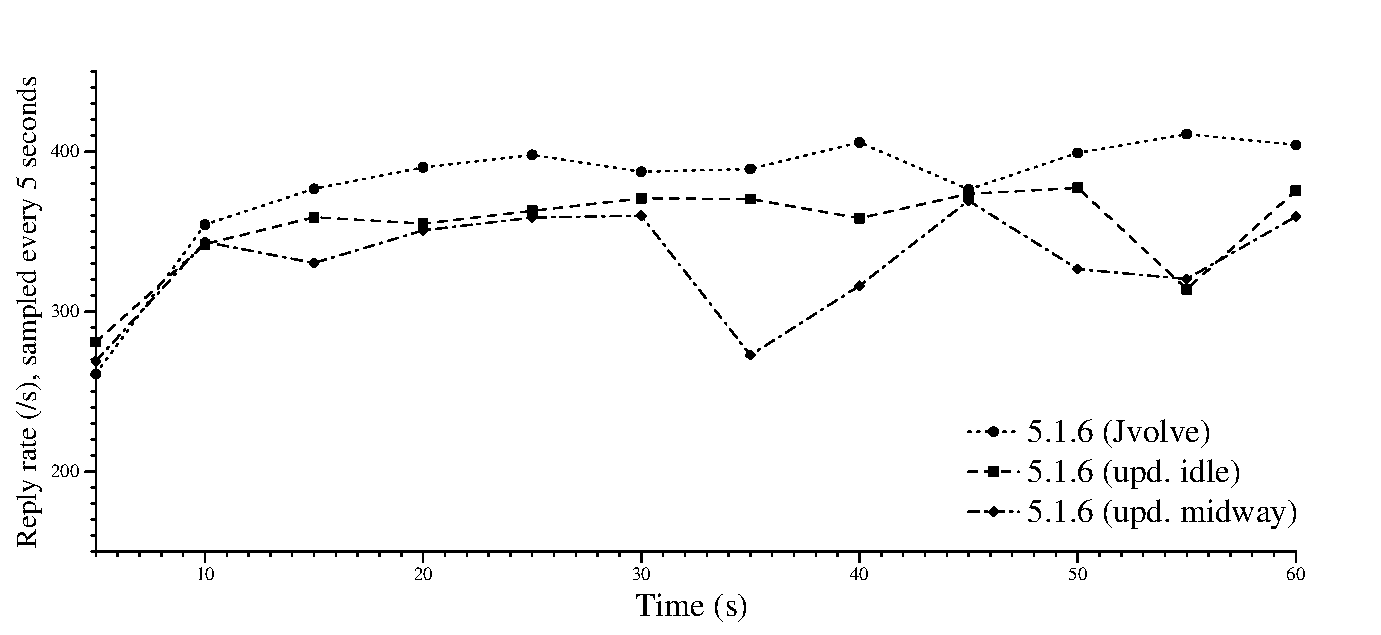
\includegraphics[width=0.5\textwidth]{jetty}
\caption{Webserver request rate over time\label{fig:jetty}}
\label{fig:jetty-rate}
\end{center}
\end{figure}

\subsection{Microbenchmarks}
\label{subsec:microbench}

The two factors that determine \DSU{} update time are the time to
perform a GC, determined by the number of objects, and the time to run
object transformers, determined by the fraction of objects being
updated. To measure the costs of each, we devised a simple
microbenchmark that creates objects and transforms a specified
fraction of these objects when a \DSU{} update is triggered. The
microbenchmark has two simple classes, \texttt{Change} and
\texttt{NoChange}.  Both start with a single integer field.  The
update adds another integer field to \texttt{Change}.  The
user-provided object transformation function copies the first field and
initializes the new field to zero.  The benchmark contains two arrays,
one for \texttt{Change} objects and one for \texttt{NoChange} objects.
We measure the cost of performing an update while varying the total
number of objects and the fraction of objects of each type.

Table~\ref{tab:microbench} shows the \DSU{} pause time for 1000 to 100000
objects (the rows) while varying the fraction of the objects that are of
type \texttt{Change} (the columns).  The first group of rows measures the
total pause time, the second group measures the portion of this time due to
running transformer functions, and the final group measures the portion of
this time due to running the garbage collector.  The first column of the
table shows that there is large fixed cost of performing a whole heap
collection even for a small number of objects.  This time includes the time
to stop the running threads and perform other setup.  As we move right in
the table, we can see that the cost of object transformation can outweigh
the cost of the garbage collection by quite a bit. Also, with more objects
to be transformed, the time to run object transformation functions
increases non-linearly, because of caching effects.

The highly optimized original copying sequence does a \texttt{memcopy}, whereas
our transformer functions use reflection and copy one field at a time.
For each transformed object, \DSU{} looks up and invokes an object's
\texttt{jvolve\_object} function using reflection, and then copies
each of the fields one by one.  The cost of reflection could be
reduced by caching the lookup, but a na\"ively compiled field-by-field
copy is much slower than the collector's highly-optimized copying loop.
Note however that the number of transformed objects in our actual
benchmarks was usually very low, less than 25 objects in the
applications we considered, as illustrated by Jetty pause times reported
above.

% \begin{verbatim}
% Total DSU Pause
%               0.00    0.10    0.20    0.30    0.40    0.50    0.60    0.70    0.80    0.90    1.00
%       1000  538.96  540.57  587.53  554.98  552.78  550.44  561.87  557.66  564.31  567.02  773.40
%      10000  529.42  584.29  597.35  624.16  647.52  675.41  721.26  738.99  811.14  773.39  799.17
%      50000  379.79  462.63  542.68  622.79  702.85  785.25  867.00 1536.62 1779.80 2020.53    None
%     100000  377.46  588.79  703.45  862.07 1777.40    None    None    None    None    None    None
%     500000  380.02 2468.65    None    None    None    None    None    None    None    None    None
%    1000000  405.53    None    None    None    None    None    None    None    None    None    None
% 
% Running transformation functions
%               0.00    0.10    0.20    0.30    0.40    0.50    0.60    0.70    0.80    0.90    1.00
%       1000    0.24    2.29    3.93    5.05    6.60    7.72    8.95   10.47   11.78   13.15   19.92
%      10000    0.24   14.64   28.45   42.66   58.38   70.13   84.34  109.72  114.00  125.96  140.16
%      50000    0.18   43.92   87.46  132.97  177.81  220.91  263.90  901.65 1108.51 1312.36    None
%     100000    0.18   96.34  175.59  262.64 1106.61    None    None    None    None    None    None
%     500000    0.17 1649.37    None    None    None    None    None    None    None    None    None
%    1000000    0.17    None    None    None    None    None    None    None    None    None    None
% 
% Garbage collection
%               0.00    0.10    0.20    0.30    0.40    0.50    0.60    0.70    0.80    0.90    1.00
%       1000  535.50  531.06  575.74  542.62  538.93  535.42  545.64  540.06  545.20  546.65  743.59
%      10000  525.84  562.48  561.50  574.23  581.97  598.06  629.68  622.11  689.90  640.29  651.72
%      50000  377.46  414.06  450.64  485.18  520.44  559.70  598.41  630.29  666.66  703.40    None
%     100000  375.16  487.49  523.03  594.53  665.91    None    None    None    None    None    None
%     500000  377.71  813.98    None    None    None    None    None    None    None    None    None
%    1000000  403.19    None    None    None    None    None    None    None    None    None    None
% \end{verbatim}

% \begin{verbatim}
% Jetty-5.1.10 - 5 January 2006
% slloccount: 44102 lines
%  + Fixed path aliasing with // on windows.
%  + Fix for AJP13 with multiple headers
%  + Fix for AJP13 with encoded path
%  + Remove null dispatch attributes from getAttributeNames
%  + Put POST content default back to iso_8859_1. GET is UTF-8 still
% 
% Jetty-5.1.9 - 7 December 2005
% slloccount: 44084 lines
%  + Fixed wantClientAuth(false) overriding netClientAuth(true) 
% 
% Jetty-5.1.8 - 7 December 2005
% slloccount: 44082 lines
%  + Fixed space in URL issued created in 5.1.6
% 
% Jetty-5.1.7 - 7 December 2005
% slloccount: 44081 lines
%  + Improved collection of statistics
%  + Better support for requst encoding.
% 
% Jetty-5.1.6 - 18 November 2005
% slloccount: 43948 lines
%  + Fixed JSP visibility security issue.
%  + Improved jetty-web.xml access to org.mortbay classes.
% 
% Jetty-5.1.5 - 10 November 2005
% slloccount: 44027 lines
%  + Improved shutdown hook
%  + Improved URL Decoding
%  + Improved mapping of JSP files.
% 
% Jetty-5.1.4 - 5 June 2005
% slloccount: 43578 lines
%  + Fixed FTP close issue.
%  + setup MX4J with JDK1.5 in start.config
%  + set classloader during webapp doStop
%  + NPE protection in ThreadedServer
%  + ModelMBean handles null signatures
%  + Change JAAS impl to be more flexible on finding roles
% 
% Jetty-5.1.3 - 7 April 2005
% slloccount: 43612 lines
%  + Some minor code janitorial services
% 
% Jetty-5.1.2 - 18 January 2005
% slloccount: 43277 lines
%  + Added id and ref support to XmlConfiguration
%  + Cleaned up AbstractSessionManager synchronization.
%  + Fixed potential concurrent login problem with JAAS
%  + Apply patch #1103953
% 
% Jetty-5.1.1 - 1 December 2004
% slloccount: 43073 lines
%  + Changes to key pair handling for SSL.
% 
% Jetty-5.1.0 - 14 November 2004
% slloccount: 42981 lines
% \end{verbatim}

% vim:ft=tex:spell:

\section{Future Work}
\ShowTOC
\begin{frame}{Looking ahead}%{A Sub-title is optional}
\begin{center}
\begin{Huge}
What's in the path towards mainstream adoption?
\end{Huge}
\end{center}
\end{frame}

\begin{frame}{Safety}%{A Sub-title is optional}
\begin{itemize}
\item Currently, we guarantee type safety. Can we do more?
\item Safe behavior in a general context is undecidable \cite{Gupta94}
\item Divide program into transactions, ensure they are version consistent
\cite{neamtiu08context}
\item Exhaustively testing updates
\end{itemize}
\end{frame}

\begin{frame}{Flexibility}%{A Sub-title is optional}
\begin{itemize}
\item Supporting every possible update is not a goal
\item Support most of the updates that occur in practice
\item Large and complex applications and updates
\item Understand update semantics from refactorings
\end{itemize}
\end{frame}

\begin{frame}{Efficiency}%{A Sub-title is optional}
\begin{itemize}
\item Update time roughly proportional to GC time
\item Semi-space GC is not practical
\item We have two requirements
  \begin{itemize}
  \item Copying objects
  \item Full-heap collection
  \end{itemize}
\item Other collectors? Concurrent collectors?
\end{itemize}
\end{frame}

\section{Conclusion}
% \ShowTOC

% \begin{frame}{Future work}%{A Sub-title is optional}
% \begin{itemize}
% \item Baby steps towards using static analysis towards asserting safety of
% updates
% \item Restricting update points based on semantics of the update
% \item How can we show that these update points are indeed safe?
% \end{itemize}
% \end{frame}

\begin{frame}{Conclusion}%{A Sub-title is optional}
\begin{itemize}
\item \DSU{}, a Java VM with support for Dynamic Software Updating
\item Most-featured, best-performing DSU system for Java
\item Naturally extends existing VM services
\item Supports about two years worth of updates
\end{itemize}
\begin{block}{}
\emph{Dynamic software updating in managed languages can be achieved in a
safe, flexible and efficient manner.}
\end{block}
\begin{center}
Source code and other information:
\url{http://www.cs.utexas.edu/~suriya/jvolve}
% Also available in the Jikes
% RVM research archive.
\end{center}
\end{frame}

% \begin{frame}{Research plan}%{A Sub-title is optional}
% \begin{center}
% \begin{large}
% Bridge the gap between static and dynamic languages
% \end{large}
% \end{center}
% \begin{itemize}
% \item Static Languages: Java, C\#
%   \begin{itemize}
%   \item Compile-time type safety
%   \item Static analysis
%   \item High performance VMs
%   \end{itemize}
% \item Dynamic Languages: Python, Ruby
%   \begin{itemize}
%   \item Expressive
%   \item Concise programs, easy to write/understand
%   \item No compile-time guarantees
%   \end{itemize}
% \end{itemize}
% \begin{center}
% \begin{large}
% Improved safety and performance of Dynamic languages
% \end{large}
% \end{center}
% \end{frame}
% 
% \begin{frame}{Solutions}%{A Sub-title is optional}
% \begin{itemize}
% \item Diamondback Ruby: Static type checking for Ruby
% \item Languages targeting the JVM: Clojure, Groovy, etc.
% \item Dynamic Language VMs: Unladen Swallow, PyPy
% \item Gradual typing
% \item DaVinci project: Dynamic language support in JVM
% \item Static Typing Where Possible, Dynamic Typing When Needed
% \end{itemize}
% \end{frame}
% 
% \begin{frame}{Conclusion}%{A Sub-title is optional}
% \begin{itemize}
% \item Work towards improving the robustness of software systems
% \item Current work: A VM-based Dynamic Software Updating solution
% \item In the future: Robust Dynamic Languages
% \end{itemize}
% \end{frame}

\appendix
\begin{frame}[allowframebreaks]{References}%{A Sub-title is optional}
\bibliographystyle{apalike}
\bibliography{paper.bib}
\end{frame}

\begin{frame}{Acknowledgements}%{A Sub-title is optional}
\begin{itemize}
\item Iulian Neamtiu
\item \JikesRVM{} community, Mike Bond, David Grove, Filip Pizlo
\item NSF CNS-0346989, NSF CCF-0811524, NSF CNS-0719966, NSF CCF-0429859,
Intel, IBM, CISCO, and Microsoft
\end{itemize}
\end{frame}

\begin{frame}{}%{A Sub-title is optional}
  \begin{center}
    {\Huge Thank you}
  \end{center}
\end{frame}

% \appendix
% \begin{frame}[allowframebreaks]{References}%{A Sub-title is optional}
% \bibliographystyle{apalike}
% \bibliography{paper.bib}
% \end{frame}


\end{document}
